\documentclass[twoside]{book}

% Packages required by doxygen
\usepackage{fixltx2e}
\usepackage{calc}
\usepackage{doxygen}
\usepackage[export]{adjustbox} % also loads graphicx
\usepackage{graphicx}
\usepackage[utf8]{inputenc}
\usepackage{makeidx}
\usepackage{multicol}
\usepackage{multirow}
\PassOptionsToPackage{warn}{textcomp}
\usepackage{textcomp}
\usepackage[nointegrals]{wasysym}
\usepackage[table]{xcolor}

% NLS support packages
\usepackage[french]{babel}

% Font selection
\usepackage[T1]{fontenc}
\usepackage[scaled=.90]{helvet}
\usepackage{courier}
\usepackage{amssymb}
\usepackage{sectsty}
\renewcommand{\familydefault}{\sfdefault}
\allsectionsfont{%
  \fontseries{bc}\selectfont%
  \color{darkgray}%
}
\renewcommand{\DoxyLabelFont}{%
  \fontseries{bc}\selectfont%
  \color{darkgray}%
}
\newcommand{\+}{\discretionary{\mbox{\scriptsize$\hookleftarrow$}}{}{}}

% Page & text layout
\usepackage{geometry}
\geometry{%
  a4paper,%
  top=2.5cm,%
  bottom=2.5cm,%
  left=2.5cm,%
  right=2.5cm%
}
\tolerance=750
\hfuzz=15pt
\hbadness=750
\setlength{\emergencystretch}{15pt}
\setlength{\parindent}{0cm}
\setlength{\parskip}{3ex plus 2ex minus 2ex}
\makeatletter
\renewcommand{\paragraph}{%
  \@startsection{paragraph}{4}{0ex}{-1.0ex}{1.0ex}{%
    \normalfont\normalsize\bfseries\SS@parafont%
  }%
}
\renewcommand{\subparagraph}{%
  \@startsection{subparagraph}{5}{0ex}{-1.0ex}{1.0ex}{%
    \normalfont\normalsize\bfseries\SS@subparafont%
  }%
}
\makeatother

% Headers & footers
\usepackage{fancyhdr}
\pagestyle{fancyplain}
\fancyhead[LE]{\fancyplain{}{\bfseries\thepage}}
\fancyhead[CE]{\fancyplain{}{}}
\fancyhead[RE]{\fancyplain{}{\bfseries\leftmark}}
\fancyhead[LO]{\fancyplain{}{\bfseries\rightmark}}
\fancyhead[CO]{\fancyplain{}{}}
\fancyhead[RO]{\fancyplain{}{\bfseries\thepage}}
\fancyfoot[LE]{\fancyplain{}{}}
\fancyfoot[CE]{\fancyplain{}{}}
\fancyfoot[RE]{\fancyplain{}{\bfseries\scriptsize Généré par Doxygen }}
\fancyfoot[LO]{\fancyplain{}{\bfseries\scriptsize Généré par Doxygen }}
\fancyfoot[CO]{\fancyplain{}{}}
\fancyfoot[RO]{\fancyplain{}{}}
\renewcommand{\footrulewidth}{0.4pt}
\renewcommand{\chaptermark}[1]{%
  \markboth{#1}{}%
}
\renewcommand{\sectionmark}[1]{%
  \markright{\thesection\ #1}%
}

% Indices & bibliography
\usepackage{natbib}
\usepackage[titles]{tocloft}
\setcounter{tocdepth}{3}
\setcounter{secnumdepth}{5}
\makeindex

% Hyperlinks (required, but should be loaded last)
\usepackage{ifpdf}
\ifpdf
  \usepackage[pdftex,pagebackref=true]{hyperref}
\else
  \usepackage[ps2pdf,pagebackref=true]{hyperref}
\fi
\hypersetup{%
  colorlinks=true,%
  linkcolor=blue,%
  citecolor=blue,%
  unicode%
}

% Custom commands
\newcommand{\clearemptydoublepage}{%
  \newpage{\pagestyle{empty}\cleardoublepage}%
}

\usepackage{caption}
\captionsetup{labelsep=space,justification=centering,font={bf},singlelinecheck=off,skip=4pt,position=top}

%===== C O N T E N T S =====

\begin{document}

% Titlepage & ToC
\hypersetup{pageanchor=false,
             bookmarksnumbered=true,
             pdfencoding=unicode
            }
\pagenumbering{alph}
\begin{titlepage}
\vspace*{7cm}
\begin{center}%
{\Large Pac\+Man\+Doc }\\
\vspace*{1cm}
{\large Généré par Doxygen 1.8.13}\\
\end{center}
\end{titlepage}
\clearemptydoublepage
\pagenumbering{roman}
\tableofcontents
\clearemptydoublepage
\pagenumbering{arabic}
\hypersetup{pageanchor=true}

%--- Begin generated contents ---
\chapter{Index hiérarchique}
\section{Hiérarchie des classes}
Cette liste d\textquotesingle{}héritage est classée approximativement par ordre alphabétique \+:\begin{DoxyCompactList}
\item \contentsline{section}{Matrice}{\pageref{class_matrice}}{}
\item Mono\+Behaviour\begin{DoxyCompactList}
\item \contentsline{section}{Button\+Script}{\pageref{class_button_script}}{}
\item \contentsline{section}{Camera\+Behavior}{\pageref{class_camera_behavior}}{}
\item \contentsline{section}{Color\+Script}{\pageref{class_color_script}}{}
\item \contentsline{section}{Grid\+Move}{\pageref{class_grid_move}}{}
\item \contentsline{section}{I\+O\+With\+Input\+Field}{\pageref{class_i_o_with_input_field}}{}
\item \contentsline{section}{Quit\+On\+Click}{\pageref{class_quit_on_click}}{}
\item \contentsline{section}{Selection\+Box}{\pageref{class_selection_box}}{}
\item \contentsline{section}{Targeting\+Move}{\pageref{class_targeting_move}}{}
\item \contentsline{section}{Tile}{\pageref{class_tile}}{}
\item \contentsline{section}{Tile\+Editor}{\pageref{class_tile_editor}}{}
\end{DoxyCompactList}
\item Object\begin{DoxyCompactList}
\item \contentsline{section}{Tile\+Matrix}{\pageref{class_tile_matrix}}{}
\end{DoxyCompactList}
\end{DoxyCompactList}

\chapter{Index des classes}
\section{Liste des classes}
Liste des classes, structures, unions et interfaces avec une brève description \+:\begin{DoxyCompactList}
\item\contentsline{section}{\hyperlink{class_button_script}{Button\+Script} }{\pageref{class_button_script}}{}
\item\contentsline{section}{\hyperlink{class_camera_behavior}{Camera\+Behavior} }{\pageref{class_camera_behavior}}{}
\item\contentsline{section}{\hyperlink{class_color_script}{Color\+Script} }{\pageref{class_color_script}}{}
\item\contentsline{section}{\hyperlink{class_grid_move}{Grid\+Move} }{\pageref{class_grid_move}}{}
\item\contentsline{section}{\hyperlink{class_i_o_with_input_field}{I\+O\+With\+Input\+Field} }{\pageref{class_i_o_with_input_field}}{}
\item\contentsline{section}{\hyperlink{class_matrice}{Matrice} \\*La class \hyperlink{class_matrice}{Matrice} permet de modifier des matrice ainsi que de les charger/sauvegarder dans des fichiers. }{\pageref{class_matrice}}{}
\item\contentsline{section}{\hyperlink{class_quit_on_click}{Quit\+On\+Click} }{\pageref{class_quit_on_click}}{}
\item\contentsline{section}{\hyperlink{class_selection_box}{Selection\+Box} }{\pageref{class_selection_box}}{}
\item\contentsline{section}{\hyperlink{class_targeting_move}{Targeting\+Move} }{\pageref{class_targeting_move}}{}
\item\contentsline{section}{\hyperlink{class_tile}{Tile} }{\pageref{class_tile}}{}
\item\contentsline{section}{\hyperlink{class_tile_editor}{Tile\+Editor} }{\pageref{class_tile_editor}}{}
\item\contentsline{section}{\hyperlink{class_tile_matrix}{Tile\+Matrix} \\*La class \hyperlink{class_tile_matrix}{Tile\+Matrix} permet de modifier des Matrices de Tuiles ainsi que de les charger/sauvegarder dans des fichiers. }{\pageref{class_tile_matrix}}{}
\end{DoxyCompactList}

\chapter{Documentation des classes}
\hypertarget{class_button_script}{}\section{Référence de la classe Button\+Script}
\label{class_button_script}\index{Button\+Script@{Button\+Script}}
Graphe d\textquotesingle{}héritage de Button\+Script\+:\begin{figure}[H]
\begin{center}
\leavevmode
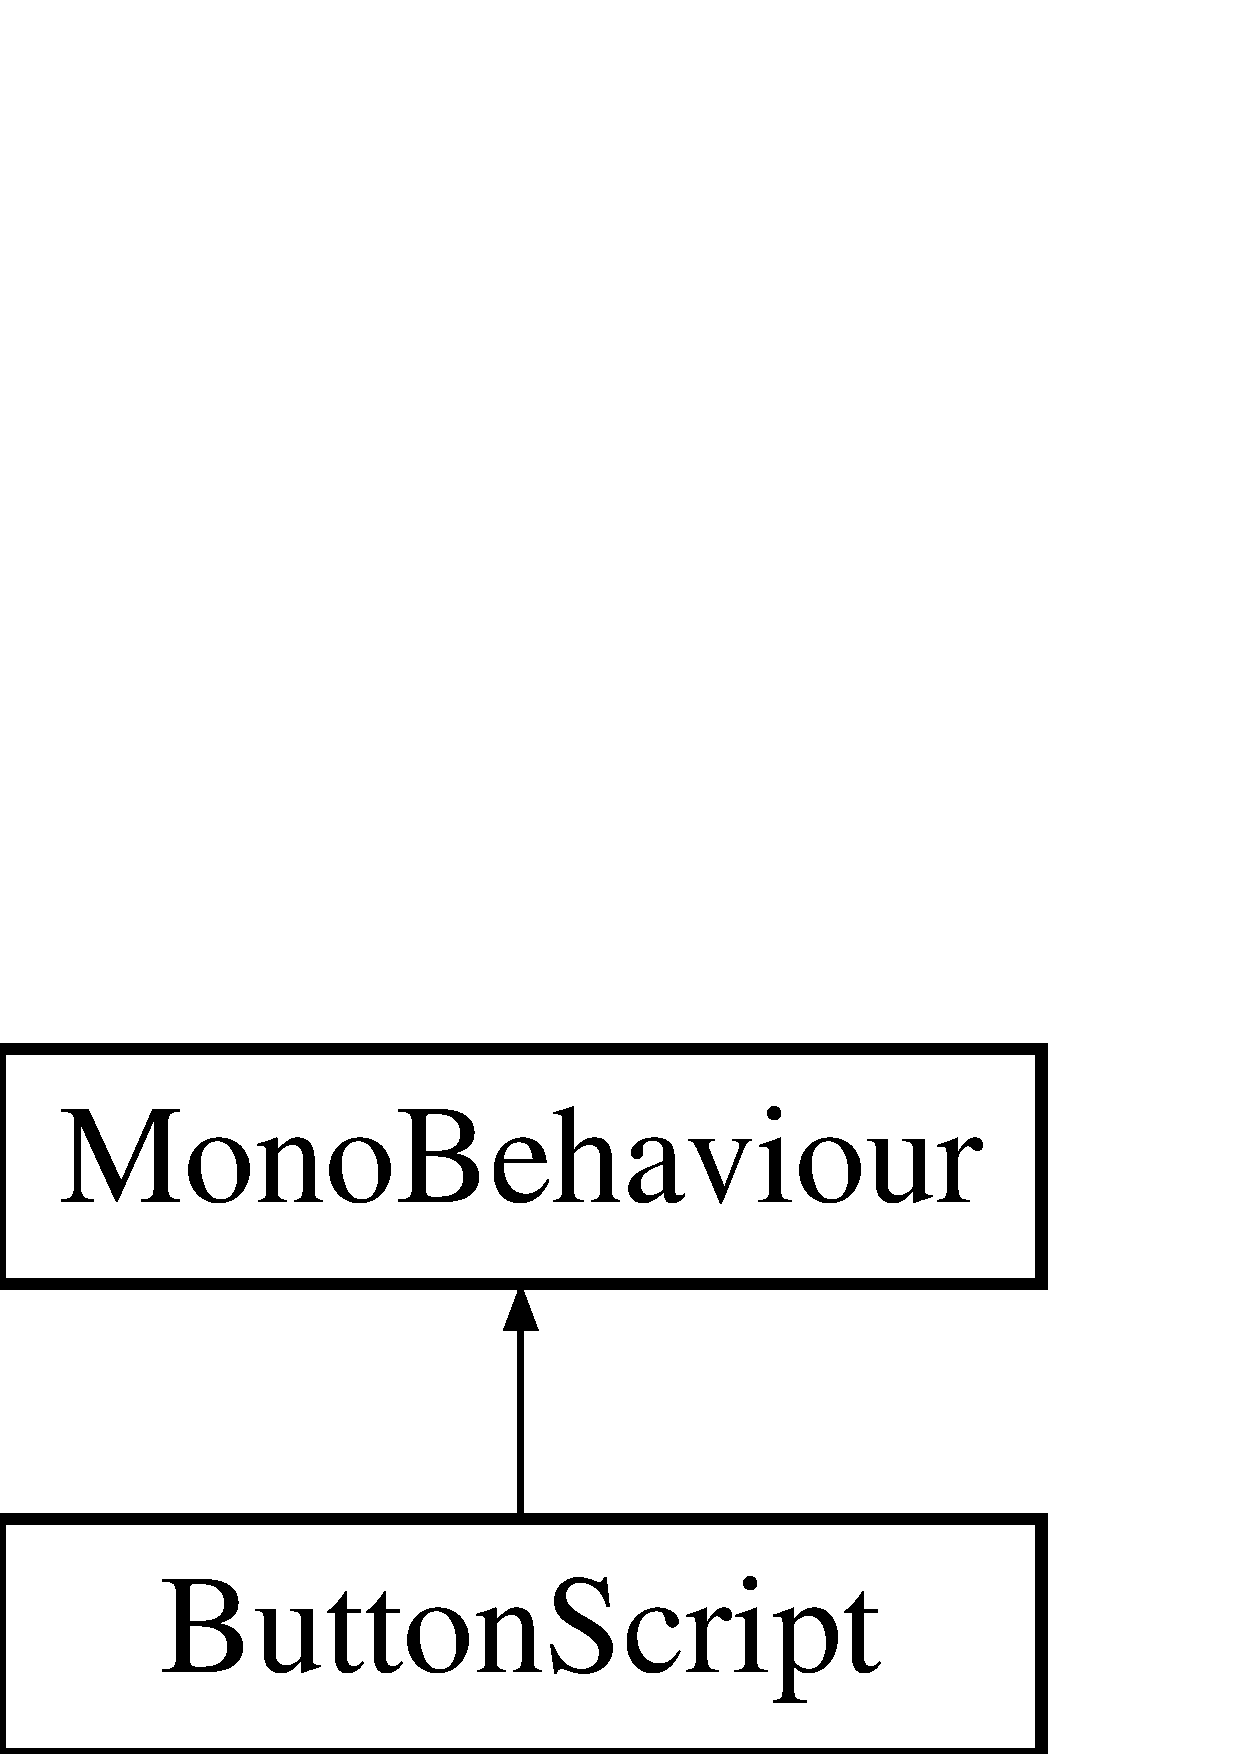
\includegraphics[height=2.000000cm]{class_button_script}
\end{center}
\end{figure}
\subsection*{Fonctions membres publiques}
\begin{DoxyCompactItemize}
\item 
\mbox{\Hypertarget{class_button_script_ab6ae2731d924263b61652a6d9e0969e2}\label{class_button_script_ab6ae2731d924263b61652a6d9e0969e2}} 
void {\bfseries change\+Text} ()
\end{DoxyCompactItemize}
\subsection*{Attributs publics}
\begin{DoxyCompactItemize}
\item 
\mbox{\Hypertarget{class_button_script_ab706f85e9e0c98764c3a1e4b113dc3f1}\label{class_button_script_ab706f85e9e0c98764c3a1e4b113dc3f1}} 
Text {\bfseries mytext} = null
\item 
\mbox{\Hypertarget{class_button_script_a1f6ec0cc79a94c93661780668ac8c173}\label{class_button_script_a1f6ec0cc79a94c93661780668ac8c173}} 
int {\bfseries counter} = 0
\end{DoxyCompactItemize}


La documentation de cette classe a été générée à partir du fichier suivant \+:\begin{DoxyCompactItemize}
\item 
Interface/Button\+Script.\+cs\end{DoxyCompactItemize}

\hypertarget{class_camera_behavior}{}\section{Référence de la classe Camera\+Behavior}
\label{class_camera_behavior}\index{Camera\+Behavior@{Camera\+Behavior}}
Graphe d\textquotesingle{}héritage de Camera\+Behavior\+:\begin{figure}[H]
\begin{center}
\leavevmode
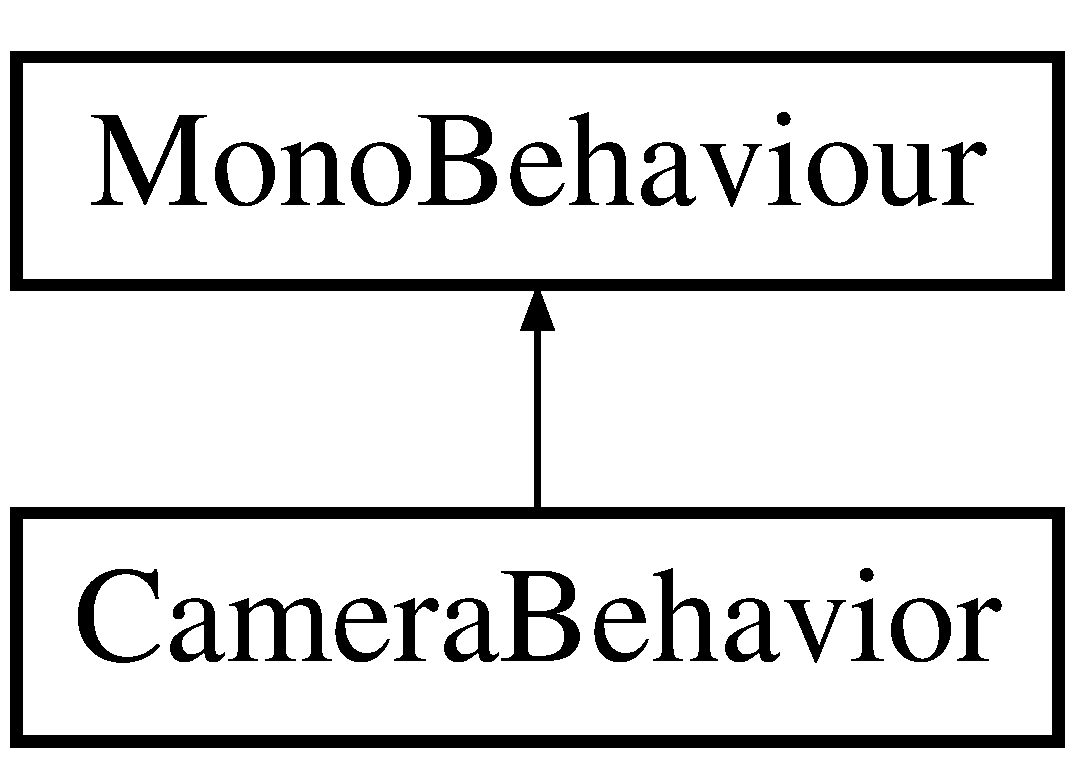
\includegraphics[height=2.000000cm]{class_camera_behavior}
\end{center}
\end{figure}
\subsection*{Fonctions membres publiques}
\begin{DoxyCompactItemize}
\item 
\mbox{\Hypertarget{class_camera_behavior_a9726b2f987d9b7b302a04edb5340a5fc}\label{class_camera_behavior_a9726b2f987d9b7b302a04edb5340a5fc}} 
void {\bfseries Fixed\+Camera} (bool is\+Fixed)
\end{DoxyCompactItemize}
\subsection*{Attributs publics}
\begin{DoxyCompactItemize}
\item 
\mbox{\Hypertarget{class_camera_behavior_aa519801079199f95d58fe9da626a8011}\label{class_camera_behavior_aa519801079199f95d58fe9da626a8011}} 
float {\bfseries scroll\+Speed} = 15.\+0f
\end{DoxyCompactItemize}


La documentation de cette classe a été générée à partir du fichier suivant \+:\begin{DoxyCompactItemize}
\item 
Interface/Camera\+Behavior.\+cs\end{DoxyCompactItemize}

\hypertarget{class_color_script}{}\section{Référence de la classe Color\+Script}
\label{class_color_script}\index{Color\+Script@{Color\+Script}}
Graphe d\textquotesingle{}héritage de Color\+Script\+:\begin{figure}[H]
\begin{center}
\leavevmode
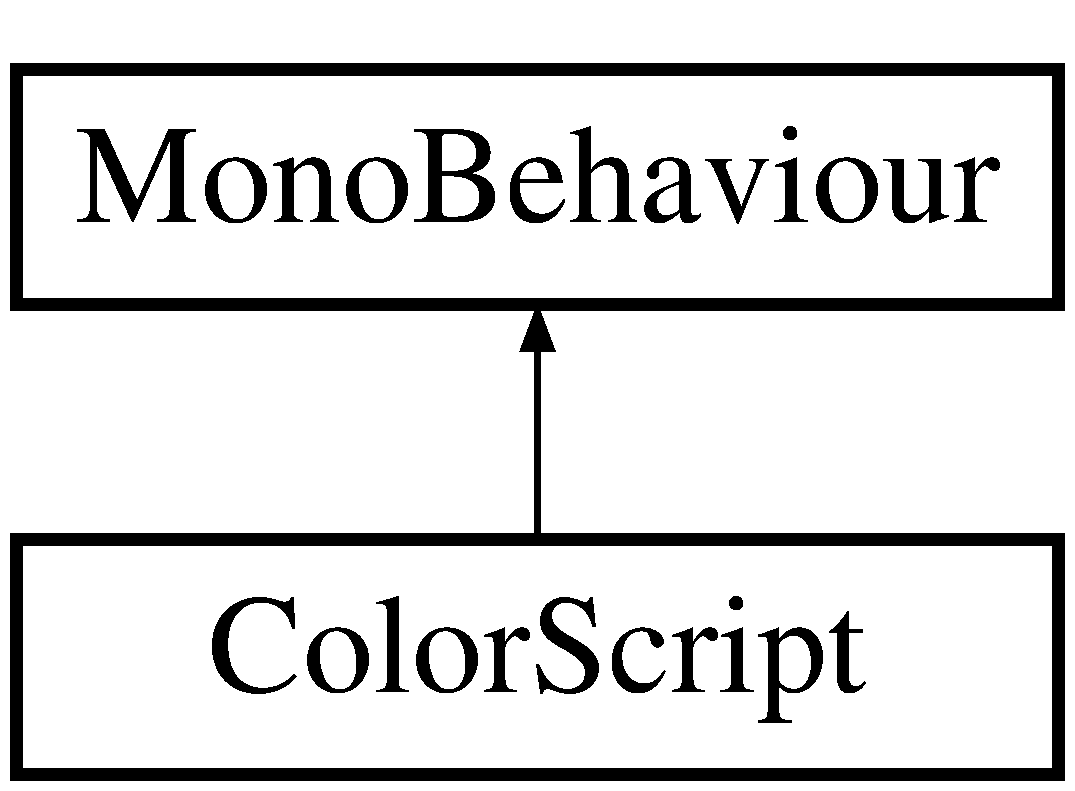
\includegraphics[height=2.000000cm]{class_color_script}
\end{center}
\end{figure}
\subsection*{Fonctions membres publiques}
\begin{DoxyCompactItemize}
\item 
\mbox{\Hypertarget{class_color_script_a506f41b4b9b1d22d00c7e3c66e11289c}\label{class_color_script_a506f41b4b9b1d22d00c7e3c66e11289c}} 
void {\bfseries Change\+Color} ()
\item 
\mbox{\Hypertarget{class_color_script_a5e63e47a62d8df19bfaa819a442065e5}\label{class_color_script_a5e63e47a62d8df19bfaa819a442065e5}} 
void {\bfseries Change\+Color\+If\+Normal} ()
\item 
\mbox{\Hypertarget{class_color_script_a16c83ff93b5bffef7ef92d81cf8216e2}\label{class_color_script_a16c83ff93b5bffef7ef92d81cf8216e2}} 
void {\bfseries Change\+Color\+If\+Diferrent} ()
\end{DoxyCompactItemize}


La documentation de cette classe a été générée à partir du fichier suivant \+:\begin{DoxyCompactItemize}
\item 
Interface/Color\+Script.\+cs\end{DoxyCompactItemize}

\hypertarget{class_grid_move}{}\section{Référence de la classe Grid\+Move}
\label{class_grid_move}\index{Grid\+Move@{Grid\+Move}}
Graphe d\textquotesingle{}héritage de Grid\+Move\+:\begin{figure}[H]
\begin{center}
\leavevmode
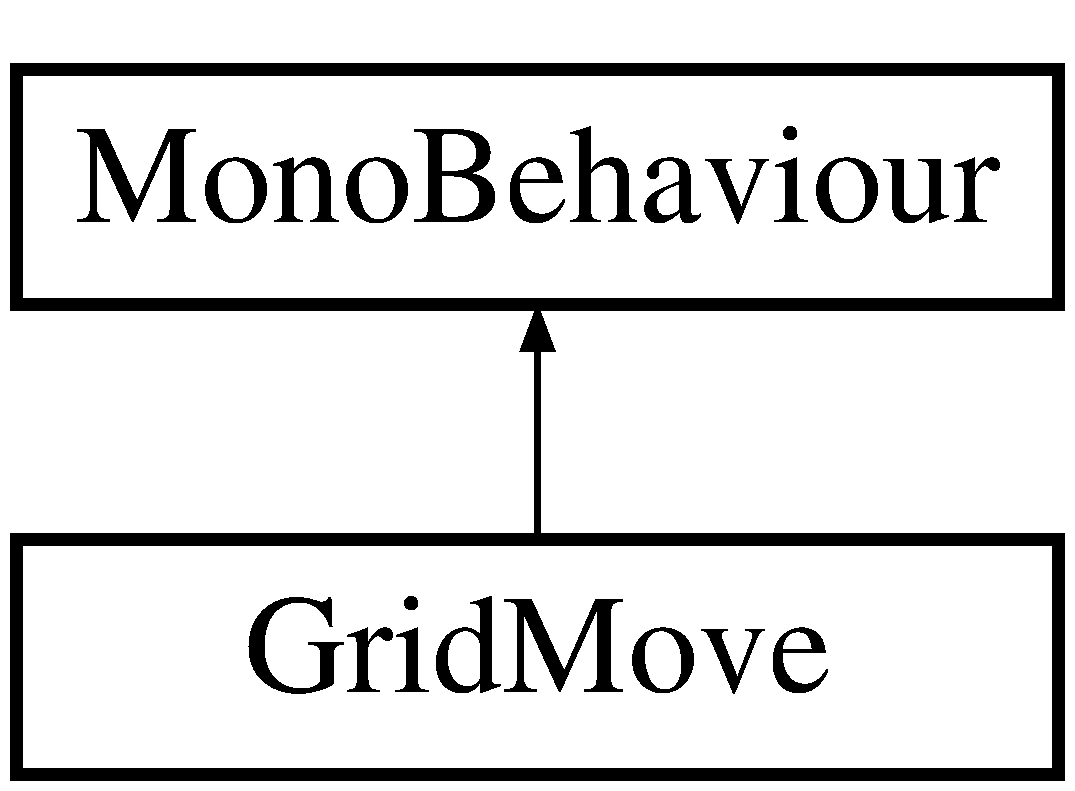
\includegraphics[height=2.000000cm]{class_grid_move}
\end{center}
\end{figure}
\subsection*{Attributs publics}
\begin{DoxyCompactItemize}
\item 
\mbox{\Hypertarget{class_grid_move_acb81136481e8d127f6910eb627f9d824}\label{class_grid_move_acb81136481e8d127f6910eb627f9d824}} 
float {\bfseries speed} = 1.\+0f
\item 
\mbox{\Hypertarget{class_grid_move_a2cf48c98cc973e87ede684a994be0b8d}\label{class_grid_move_a2cf48c98cc973e87ede684a994be0b8d}} 
float {\bfseries blocksize} = 0.\+24f
\item 
\mbox{\Hypertarget{class_grid_move_a8aab00834e6f2c01b784f43e38704df0}\label{class_grid_move_a8aab00834e6f2c01b784f43e38704df0}} 
string {\bfseries first\+Direction} = \char`\"{}aucune\char`\"{}
\end{DoxyCompactItemize}


La documentation de cette classe a été générée à partir du fichier suivant \+:\begin{DoxyCompactItemize}
\item 
Move/Grid\+Move.\+cs\end{DoxyCompactItemize}

\hypertarget{class_i_o_with_input_field}{}\section{Référence de la classe I\+O\+With\+Input\+Field}
\label{class_i_o_with_input_field}\index{I\+O\+With\+Input\+Field@{I\+O\+With\+Input\+Field}}
Graphe d\textquotesingle{}héritage de I\+O\+With\+Input\+Field\+:\begin{figure}[H]
\begin{center}
\leavevmode
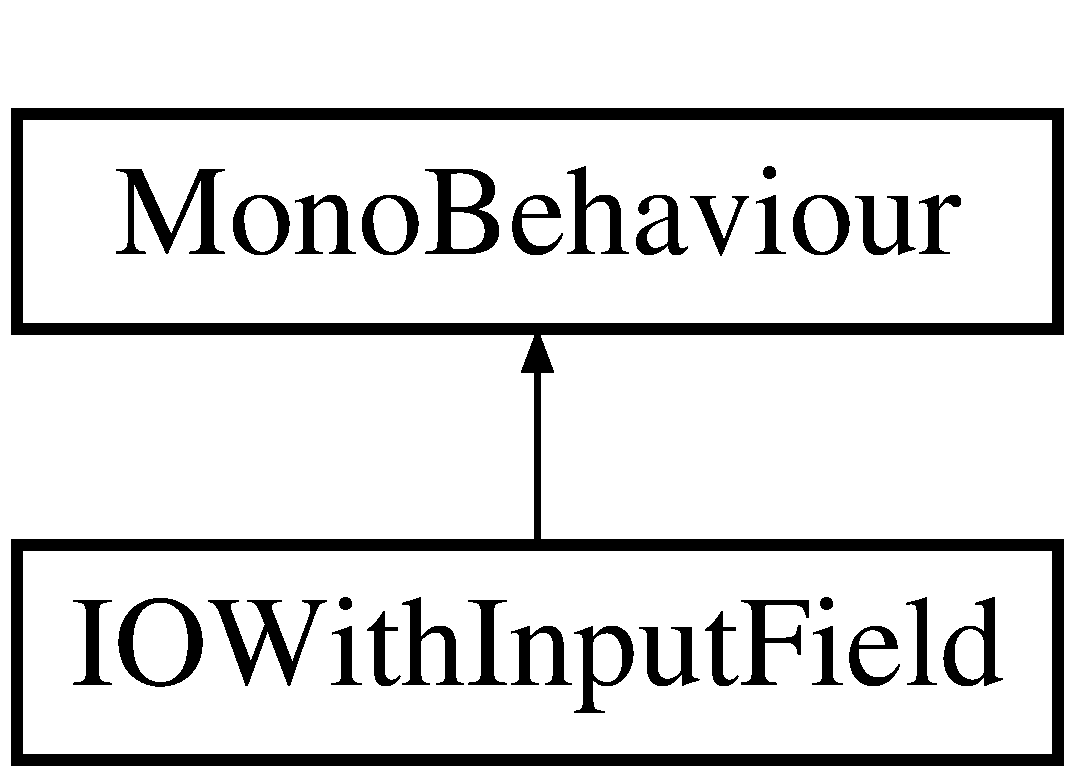
\includegraphics[height=2.000000cm]{class_i_o_with_input_field}
\end{center}
\end{figure}
\subsection*{Fonctions membres publiques}
\begin{DoxyCompactItemize}
\item 
\mbox{\Hypertarget{class_i_o_with_input_field_a5d6a1f8b94ecea4fc82fd97f297e0d77}\label{class_i_o_with_input_field_a5d6a1f8b94ecea4fc82fd97f297e0d77}} 
void {\bfseries Saving} ()
\item 
\mbox{\Hypertarget{class_i_o_with_input_field_a3f02c4fda3cc9bf49605a35a08c78fcd}\label{class_i_o_with_input_field_a3f02c4fda3cc9bf49605a35a08c78fcd}} 
void {\bfseries Charging} ()
\item 
\mbox{\Hypertarget{class_i_o_with_input_field_a02e95196cec3127f0b8977bd9a60f159}\label{class_i_o_with_input_field_a02e95196cec3127f0b8977bd9a60f159}} 
void {\bfseries Save\+Or\+Load\+Lvl\+With\+Field} ()
\item 
\mbox{\Hypertarget{class_i_o_with_input_field_a7c92df1bf7e5e7f42bfd7bcb1afcba04}\label{class_i_o_with_input_field_a7c92df1bf7e5e7f42bfd7bcb1afcba04}} 
void {\bfseries Activate} ()
\item 
\mbox{\Hypertarget{class_i_o_with_input_field_a59aa447c2460a8e44367d10ca18aa2f1}\label{class_i_o_with_input_field_a59aa447c2460a8e44367d10ca18aa2f1}} 
void {\bfseries Desactivate} ()
\end{DoxyCompactItemize}
\subsection*{Attributs publics}
\begin{DoxyCompactItemize}
\item 
\mbox{\Hypertarget{class_i_o_with_input_field_a035182cfc25f0f5f895b19555f68f11f}\label{class_i_o_with_input_field_a035182cfc25f0f5f895b19555f68f11f}} 
Input\+Field {\bfseries Field}
\end{DoxyCompactItemize}
\subsection*{Attributs protégés}
\begin{DoxyCompactItemize}
\item 
\mbox{\Hypertarget{class_i_o_with_input_field_aa82e8c4a2116fd415d1970986860a3b9}\label{class_i_o_with_input_field_aa82e8c4a2116fd415d1970986860a3b9}} 
bool {\bfseries saving} = false
\item 
\mbox{\Hypertarget{class_i_o_with_input_field_a8a4cc7df44ff2a3aae9683e718e6edc6}\label{class_i_o_with_input_field_a8a4cc7df44ff2a3aae9683e718e6edc6}} 
bool {\bfseries charging} = false
\end{DoxyCompactItemize}


La documentation de cette classe a été générée à partir du fichier suivant \+:\begin{DoxyCompactItemize}
\item 
Interface/I\+O\+With\+Input\+Field.\+cs\end{DoxyCompactItemize}

\hypertarget{class_matrice}{}\section{Référence de la classe Matrice}
\label{class_matrice}\index{Matrice@{Matrice}}


La class \hyperlink{class_matrice}{Matrice} permet de modifier des matrice ainsi que de les charger/sauvegarder dans des fichiers.  


\subsection*{Fonctions membres publiques}
\begin{DoxyCompactItemize}
\item 
\hyperlink{class_matrice_a7281d022328e8f455eff2dc73a78593a}{Matrice} ()
\begin{DoxyCompactList}\small\item\em Constructeur par default. \end{DoxyCompactList}\item 
\hyperlink{class_matrice_af00cc9de4742a97a34d6dd3a4e5bca93}{Matrice} (int \hyperlink{class_matrice_a40c26a2a701faf2b1680886a8aeeadaf}{hauteur}, int \hyperlink{class_matrice_a01649b7f1fb32a6a8561c308a22bd22f}{largeur}, int init=0)
\begin{DoxyCompactList}\small\item\em Constructeur paramètrique. \end{DoxyCompactList}\item 
\hyperlink{class_matrice_a5a09b487960e0274a8caba85cf34397d}{Matrice} (\hyperlink{class_matrice}{Matrice} M)
\begin{DoxyCompactList}\small\item\em Constructeur par copy. \end{DoxyCompactList}\item 
void \hyperlink{class_matrice_a61f65eda2c1f1853e8f72cd25de54776}{copy} (\hyperlink{class_matrice}{Matrice} M)
\begin{DoxyCompactList}\small\item\em Copie toute les valeur et le format d\textquotesingle{}une \hyperlink{class_matrice}{Matrice} M. \end{DoxyCompactList}\item 
int \hyperlink{class_matrice_ad735382f0606ee683c761402af6f5a78}{at} (int i, int j)
\begin{DoxyCompactList}\small\item\em Accesseur en lecture des données. \end{DoxyCompactList}\item 
void \hyperlink{class_matrice_acfbf84f67a67b40c08239217caab14a9}{set\+Val} (int i, int j, int val)
\begin{DoxyCompactList}\small\item\em Accesseur en ecriture des données. \end{DoxyCompactList}\item 
int \hyperlink{class_matrice_a40c26a2a701faf2b1680886a8aeeadaf}{hauteur} ()
\begin{DoxyCompactList}\small\item\em Accesseur en lecture. \end{DoxyCompactList}\item 
int \hyperlink{class_matrice_a01649b7f1fb32a6a8561c308a22bd22f}{largeur} ()
\begin{DoxyCompactList}\small\item\em Accesseur en lecture. \end{DoxyCompactList}\item 
void \hyperlink{class_matrice_a6c119431b7a8641c5b6ea19bce336036}{add\+Ligne} (int val=0)
\begin{DoxyCompactList}\small\item\em Ajoute une Ligne à la \hyperlink{class_matrice}{Matrice}. \end{DoxyCompactList}\item 
void \hyperlink{class_matrice_a64aff02cb523d7a5db9bb268f2012444}{add\+Colonne} (int val=0)
\begin{DoxyCompactList}\small\item\em Ajoute une colonne a la matrice. \end{DoxyCompactList}\item 
void \hyperlink{class_matrice_aa90563f9897d38e422c9459de72cfc34}{set\+Ligne} (int i, int val)
\begin{DoxyCompactList}\small\item\em Accesseur en ecriture, change toute les valeur d\textquotesingle{}une ligne. \end{DoxyCompactList}\item 
void \hyperlink{class_matrice_aa8cd6d3e8e1d5250a6b56423dc61fcc4}{set\+Colonne} (int j, int val)
\begin{DoxyCompactList}\small\item\em Accesseur en ecriture, change toute les valeur d\textquotesingle{}une colonne. \end{DoxyCompactList}\item 
void \hyperlink{class_matrice_ae71605cb8df11905415a76eae31d1ad7}{replace} (int a, int b)
\begin{DoxyCompactList}\small\item\em Remplace chaque valeur \char`\"{}a\char`\"{} de la matrice par la valeur \char`\"{}b\char`\"{}. \end{DoxyCompactList}\item 
void \hyperlink{class_matrice_ad56071409baa0132735123049f27554f}{print} ()
\begin{DoxyCompactList}\small\item\em Affiche le contenu de la matrice dans la console. \end{DoxyCompactList}\item 
void \hyperlink{class_matrice_a1cf5f2836440913f2d4743ac19743ff3}{save} (string chemin)
\begin{DoxyCompactList}\small\item\em Sauvegarde toute la matrice dans un fichier. \end{DoxyCompactList}\item 
void \hyperlink{class_matrice_aee7c3766d6b49ea2cd8b7dd0eb2cfa81}{load} (string chemin, int num=0)
\begin{DoxyCompactList}\small\item\em charge une matrice contenu dans un fichier. \end{DoxyCompactList}\end{DoxyCompactItemize}
\subsection*{Attributs protégés}
\begin{DoxyCompactItemize}
\item 
List$<$ List$<$ int $>$ $>$ \hyperlink{class_matrice_af98e31a75e7e943e7fa7e59acd779a8b}{\+\_\+matrice}
\begin{DoxyCompactList}\small\item\em Liste de liste (contient les données).\end{DoxyCompactList}\item 
int \hyperlink{class_matrice_afd223a80742ca7c9c7ba6fb719289388}{\+\_\+hauteur}
\begin{DoxyCompactList}\small\item\em Hauteur du tableau.\end{DoxyCompactList}\item 
int \hyperlink{class_matrice_a6db7d42ff5538e68e3b58eec9dc44285}{\+\_\+largeur}
\begin{DoxyCompactList}\small\item\em Largeur du tableau.\end{DoxyCompactList}\end{DoxyCompactItemize}
\subsection*{Propriétés}
\begin{DoxyCompactItemize}
\item 
int \hyperlink{class_matrice_a264f2ef7eaf36019b8c84f5bca240efc}{this\mbox{[}int i, int j\mbox{]}}\hspace{0.3cm}{\ttfamily  \mbox{[}get, set\mbox{]}}
\begin{DoxyCompactList}\small\item\em Indexeur de la \hyperlink{class_matrice}{Matrice} permet un acces au données en lecture et en ecriture. \end{DoxyCompactList}\end{DoxyCompactItemize}


\subsection{Description détaillée}
La class \hyperlink{class_matrice}{Matrice} permet de modifier des matrice ainsi que de les charger/sauvegarder dans des fichiers. 



\subsection{Documentation des constructeurs et destructeur}
\mbox{\Hypertarget{class_matrice_a7281d022328e8f455eff2dc73a78593a}\label{class_matrice_a7281d022328e8f455eff2dc73a78593a}} 
\index{Matrice@{Matrice}!Matrice@{Matrice}}
\index{Matrice@{Matrice}!Matrice@{Matrice}}
\subsubsection{\texorpdfstring{Matrice()}{Matrice()}\hspace{0.1cm}{\footnotesize\ttfamily [1/3]}}
{\footnotesize\ttfamily Matrice.\+Matrice (\begin{DoxyParamCaption}{ }\end{DoxyParamCaption})}



Constructeur par default. 

\mbox{\Hypertarget{class_matrice_af00cc9de4742a97a34d6dd3a4e5bca93}\label{class_matrice_af00cc9de4742a97a34d6dd3a4e5bca93}} 
\index{Matrice@{Matrice}!Matrice@{Matrice}}
\index{Matrice@{Matrice}!Matrice@{Matrice}}
\subsubsection{\texorpdfstring{Matrice()}{Matrice()}\hspace{0.1cm}{\footnotesize\ttfamily [2/3]}}
{\footnotesize\ttfamily Matrice.\+Matrice (\begin{DoxyParamCaption}\item[{int}]{hauteur,  }\item[{int}]{largeur,  }\item[{int}]{init = {\ttfamily 0} }\end{DoxyParamCaption})}



Constructeur paramètrique. 

\mbox{\Hypertarget{class_matrice_a5a09b487960e0274a8caba85cf34397d}\label{class_matrice_a5a09b487960e0274a8caba85cf34397d}} 
\index{Matrice@{Matrice}!Matrice@{Matrice}}
\index{Matrice@{Matrice}!Matrice@{Matrice}}
\subsubsection{\texorpdfstring{Matrice()}{Matrice()}\hspace{0.1cm}{\footnotesize\ttfamily [3/3]}}
{\footnotesize\ttfamily Matrice.\+Matrice (\begin{DoxyParamCaption}\item[{\hyperlink{class_matrice}{Matrice}}]{M }\end{DoxyParamCaption})}



Constructeur par copy. 



\subsection{Documentation des fonctions membres}
\mbox{\Hypertarget{class_matrice_a64aff02cb523d7a5db9bb268f2012444}\label{class_matrice_a64aff02cb523d7a5db9bb268f2012444}} 
\index{Matrice@{Matrice}!add\+Colonne@{add\+Colonne}}
\index{add\+Colonne@{add\+Colonne}!Matrice@{Matrice}}
\subsubsection{\texorpdfstring{add\+Colonne()}{addColonne()}}
{\footnotesize\ttfamily void Matrice.\+add\+Colonne (\begin{DoxyParamCaption}\item[{int}]{val = {\ttfamily 0} }\end{DoxyParamCaption})}



Ajoute une colonne a la matrice. 


\begin{DoxyParams}{Paramètres}
{\em val} & valeur d\textquotesingle{}initialisation de la colonne \\
\hline
\end{DoxyParams}
\mbox{\Hypertarget{class_matrice_a6c119431b7a8641c5b6ea19bce336036}\label{class_matrice_a6c119431b7a8641c5b6ea19bce336036}} 
\index{Matrice@{Matrice}!add\+Ligne@{add\+Ligne}}
\index{add\+Ligne@{add\+Ligne}!Matrice@{Matrice}}
\subsubsection{\texorpdfstring{add\+Ligne()}{addLigne()}}
{\footnotesize\ttfamily void Matrice.\+add\+Ligne (\begin{DoxyParamCaption}\item[{int}]{val = {\ttfamily 0} }\end{DoxyParamCaption})}



Ajoute une Ligne à la \hyperlink{class_matrice}{Matrice}. 


\begin{DoxyParams}{Paramètres}
{\em val} & valeur d\textquotesingle{}initialisation de la colonne \\
\hline
\end{DoxyParams}
\mbox{\Hypertarget{class_matrice_ad735382f0606ee683c761402af6f5a78}\label{class_matrice_ad735382f0606ee683c761402af6f5a78}} 
\index{Matrice@{Matrice}!at@{at}}
\index{at@{at}!Matrice@{Matrice}}
\subsubsection{\texorpdfstring{at()}{at()}}
{\footnotesize\ttfamily int Matrice.\+at (\begin{DoxyParamCaption}\item[{int}]{i,  }\item[{int}]{j }\end{DoxyParamCaption})}



Accesseur en lecture des données. 


\begin{DoxyParams}{Paramètres}
{\em i} & Correspond à la ligne N°i \\
\hline
{\em j} & Correspond à la colonne N°j \\
\hline
\end{DoxyParams}
\begin{DoxyReturn}{Renvoie}
La valeur de la matrice à la ligne i et la colonne j. 
\end{DoxyReturn}
\mbox{\Hypertarget{class_matrice_a61f65eda2c1f1853e8f72cd25de54776}\label{class_matrice_a61f65eda2c1f1853e8f72cd25de54776}} 
\index{Matrice@{Matrice}!copy@{copy}}
\index{copy@{copy}!Matrice@{Matrice}}
\subsubsection{\texorpdfstring{copy()}{copy()}}
{\footnotesize\ttfamily void Matrice.\+copy (\begin{DoxyParamCaption}\item[{\hyperlink{class_matrice}{Matrice}}]{M }\end{DoxyParamCaption})}



Copie toute les valeur et le format d\textquotesingle{}une \hyperlink{class_matrice}{Matrice} M. 


\begin{DoxyParams}{Paramètres}
{\em M} & La matrice que l\textquotesingle{}on veut copier \\
\hline
\end{DoxyParams}
\mbox{\Hypertarget{class_matrice_a40c26a2a701faf2b1680886a8aeeadaf}\label{class_matrice_a40c26a2a701faf2b1680886a8aeeadaf}} 
\index{Matrice@{Matrice}!hauteur@{hauteur}}
\index{hauteur@{hauteur}!Matrice@{Matrice}}
\subsubsection{\texorpdfstring{hauteur()}{hauteur()}}
{\footnotesize\ttfamily int Matrice.\+hauteur (\begin{DoxyParamCaption}{ }\end{DoxyParamCaption})}



Accesseur en lecture. 

\begin{DoxyReturn}{Renvoie}
La hauteur de la matrice. 
\end{DoxyReturn}
\mbox{\Hypertarget{class_matrice_a01649b7f1fb32a6a8561c308a22bd22f}\label{class_matrice_a01649b7f1fb32a6a8561c308a22bd22f}} 
\index{Matrice@{Matrice}!largeur@{largeur}}
\index{largeur@{largeur}!Matrice@{Matrice}}
\subsubsection{\texorpdfstring{largeur()}{largeur()}}
{\footnotesize\ttfamily int Matrice.\+largeur (\begin{DoxyParamCaption}{ }\end{DoxyParamCaption})}



Accesseur en lecture. 

\begin{DoxyReturn}{Renvoie}
La largeur de la matrice. 
\end{DoxyReturn}
\mbox{\Hypertarget{class_matrice_aee7c3766d6b49ea2cd8b7dd0eb2cfa81}\label{class_matrice_aee7c3766d6b49ea2cd8b7dd0eb2cfa81}} 
\index{Matrice@{Matrice}!load@{load}}
\index{load@{load}!Matrice@{Matrice}}
\subsubsection{\texorpdfstring{load()}{load()}}
{\footnotesize\ttfamily void Matrice.\+load (\begin{DoxyParamCaption}\item[{string}]{chemin,  }\item[{int}]{num = {\ttfamily 0} }\end{DoxyParamCaption})}



charge une matrice contenu dans un fichier. 


\begin{DoxyParams}{Paramètres}
{\em chemin} & Le chemin du fichier que l\textquotesingle{}on veut charger \\
\hline
{\em num} & le numero de la matrice que l\textquotesingle{}on veut charger \\
\hline
\end{DoxyParams}
\mbox{\Hypertarget{class_matrice_ad56071409baa0132735123049f27554f}\label{class_matrice_ad56071409baa0132735123049f27554f}} 
\index{Matrice@{Matrice}!print@{print}}
\index{print@{print}!Matrice@{Matrice}}
\subsubsection{\texorpdfstring{print()}{print()}}
{\footnotesize\ttfamily void Matrice.\+print (\begin{DoxyParamCaption}{ }\end{DoxyParamCaption})}



Affiche le contenu de la matrice dans la console. 

\mbox{\Hypertarget{class_matrice_ae71605cb8df11905415a76eae31d1ad7}\label{class_matrice_ae71605cb8df11905415a76eae31d1ad7}} 
\index{Matrice@{Matrice}!replace@{replace}}
\index{replace@{replace}!Matrice@{Matrice}}
\subsubsection{\texorpdfstring{replace()}{replace()}}
{\footnotesize\ttfamily void Matrice.\+replace (\begin{DoxyParamCaption}\item[{int}]{a,  }\item[{int}]{b }\end{DoxyParamCaption})}



Remplace chaque valeur \char`\"{}a\char`\"{} de la matrice par la valeur \char`\"{}b\char`\"{}. 


\begin{DoxyParams}{Paramètres}
{\em a} & Valeur à chercher et remplacer \\
\hline
{\em b} & Valeur avec laquel sera remplacer \char`\"{}a\char`\"{} \\
\hline
\end{DoxyParams}
\mbox{\Hypertarget{class_matrice_a1cf5f2836440913f2d4743ac19743ff3}\label{class_matrice_a1cf5f2836440913f2d4743ac19743ff3}} 
\index{Matrice@{Matrice}!save@{save}}
\index{save@{save}!Matrice@{Matrice}}
\subsubsection{\texorpdfstring{save()}{save()}}
{\footnotesize\ttfamily void Matrice.\+save (\begin{DoxyParamCaption}\item[{string}]{chemin }\end{DoxyParamCaption})}



Sauvegarde toute la matrice dans un fichier. 


\begin{DoxyParams}{Paramètres}
{\em chemin} & Le chemin du fichier ou l\textquotesingle{}on veut sauvegarder \\
\hline
\end{DoxyParams}
\mbox{\Hypertarget{class_matrice_aa8cd6d3e8e1d5250a6b56423dc61fcc4}\label{class_matrice_aa8cd6d3e8e1d5250a6b56423dc61fcc4}} 
\index{Matrice@{Matrice}!set\+Colonne@{set\+Colonne}}
\index{set\+Colonne@{set\+Colonne}!Matrice@{Matrice}}
\subsubsection{\texorpdfstring{set\+Colonne()}{setColonne()}}
{\footnotesize\ttfamily void Matrice.\+set\+Colonne (\begin{DoxyParamCaption}\item[{int}]{j,  }\item[{int}]{val }\end{DoxyParamCaption})}



Accesseur en ecriture, change toute les valeur d\textquotesingle{}une colonne. 


\begin{DoxyParams}{Paramètres}
{\em j} & Correspond a la colonne N°j \\
\hline
{\em val} & Nouvelle valeur sur toute a la colonne j \\
\hline
\end{DoxyParams}
\mbox{\Hypertarget{class_matrice_aa90563f9897d38e422c9459de72cfc34}\label{class_matrice_aa90563f9897d38e422c9459de72cfc34}} 
\index{Matrice@{Matrice}!set\+Ligne@{set\+Ligne}}
\index{set\+Ligne@{set\+Ligne}!Matrice@{Matrice}}
\subsubsection{\texorpdfstring{set\+Ligne()}{setLigne()}}
{\footnotesize\ttfamily void Matrice.\+set\+Ligne (\begin{DoxyParamCaption}\item[{int}]{i,  }\item[{int}]{val }\end{DoxyParamCaption})}



Accesseur en ecriture, change toute les valeur d\textquotesingle{}une ligne. 


\begin{DoxyParams}{Paramètres}
{\em i} & Correspond a la ligne N°i \\
\hline
{\em val} & Nouvelle valeur sur toute a la ligne i \\
\hline
\end{DoxyParams}
\mbox{\Hypertarget{class_matrice_acfbf84f67a67b40c08239217caab14a9}\label{class_matrice_acfbf84f67a67b40c08239217caab14a9}} 
\index{Matrice@{Matrice}!set\+Val@{set\+Val}}
\index{set\+Val@{set\+Val}!Matrice@{Matrice}}
\subsubsection{\texorpdfstring{set\+Val()}{setVal()}}
{\footnotesize\ttfamily void Matrice.\+set\+Val (\begin{DoxyParamCaption}\item[{int}]{i,  }\item[{int}]{j,  }\item[{int}]{val }\end{DoxyParamCaption})}



Accesseur en ecriture des données. 


\begin{DoxyParams}{Paramètres}
{\em i} & Correspond à la ligne N°i \\
\hline
{\em j} & Correspond à la colonne N°j \\
\hline
{\em val} & Correspond à la val à changer\\
\hline
\end{DoxyParams}


\subsection{Documentation des données membres}
\mbox{\Hypertarget{class_matrice_afd223a80742ca7c9c7ba6fb719289388}\label{class_matrice_afd223a80742ca7c9c7ba6fb719289388}} 
\index{Matrice@{Matrice}!\+\_\+hauteur@{\+\_\+hauteur}}
\index{\+\_\+hauteur@{\+\_\+hauteur}!Matrice@{Matrice}}
\subsubsection{\texorpdfstring{\+\_\+hauteur}{\_hauteur}}
{\footnotesize\ttfamily int Matrice.\+\_\+hauteur\hspace{0.3cm}{\ttfamily [protected]}}



Hauteur du tableau.

\mbox{\Hypertarget{class_matrice_a6db7d42ff5538e68e3b58eec9dc44285}\label{class_matrice_a6db7d42ff5538e68e3b58eec9dc44285}} 
\index{Matrice@{Matrice}!\+\_\+largeur@{\+\_\+largeur}}
\index{\+\_\+largeur@{\+\_\+largeur}!Matrice@{Matrice}}
\subsubsection{\texorpdfstring{\+\_\+largeur}{\_largeur}}
{\footnotesize\ttfamily int Matrice.\+\_\+largeur\hspace{0.3cm}{\ttfamily [protected]}}



Largeur du tableau.

\mbox{\Hypertarget{class_matrice_af98e31a75e7e943e7fa7e59acd779a8b}\label{class_matrice_af98e31a75e7e943e7fa7e59acd779a8b}} 
\index{Matrice@{Matrice}!\+\_\+matrice@{\+\_\+matrice}}
\index{\+\_\+matrice@{\+\_\+matrice}!Matrice@{Matrice}}
\subsubsection{\texorpdfstring{\+\_\+matrice}{\_matrice}}
{\footnotesize\ttfamily List$<$List$<$int$>$ $>$ Matrice.\+\_\+matrice\hspace{0.3cm}{\ttfamily [protected]}}



Liste de liste (contient les données).



\subsection{Documentation des propriétés}
\mbox{\Hypertarget{class_matrice_a264f2ef7eaf36019b8c84f5bca240efc}\label{class_matrice_a264f2ef7eaf36019b8c84f5bca240efc}} 
\index{Matrice@{Matrice}!this\mbox{[}int i, int j\mbox{]}@{this[int i, int j]}}
\index{this\mbox{[}int i, int j\mbox{]}@{this[int i, int j]}!Matrice@{Matrice}}
\subsubsection{\texorpdfstring{this[int i, int j]}{this[int i, int j]}}
{\footnotesize\ttfamily int Matrice.\+this\mbox{[}int i, int j\mbox{]}\hspace{0.3cm}{\ttfamily [get]}, {\ttfamily [set]}}



Indexeur de la \hyperlink{class_matrice}{Matrice} permet un acces au données en lecture et en ecriture. 


\begin{DoxyParams}{Paramètres}
{\em i} & Correspond a la ligne N°i \\
\hline
{\em j} & Correspond a la colonne N°j \\
\hline
\end{DoxyParams}
\begin{DoxyReturn}{Renvoie}
La valeur que la matrice contiens à la ligne i et la colonne j 
\end{DoxyReturn}


La documentation de cette classe a été générée à partir du fichier suivant \+:\begin{DoxyCompactItemize}
\item 
Tile\+Map/Matrice.\+cs\end{DoxyCompactItemize}

\hypertarget{class_quit_on_click}{}\section{Référence de la classe Quit\+On\+Click}
\label{class_quit_on_click}\index{Quit\+On\+Click@{Quit\+On\+Click}}
Graphe d\textquotesingle{}héritage de Quit\+On\+Click\+:\begin{figure}[H]
\begin{center}
\leavevmode
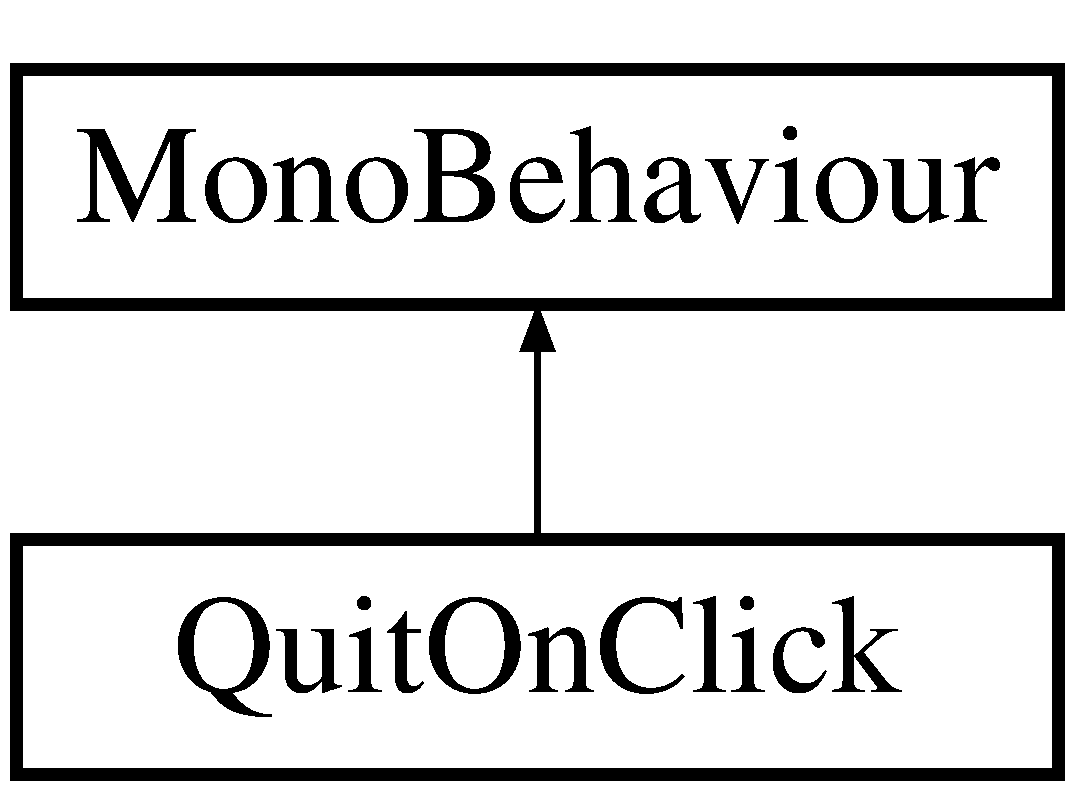
\includegraphics[height=2.000000cm]{class_quit_on_click}
\end{center}
\end{figure}
\subsection*{Fonctions membres publiques}
\begin{DoxyCompactItemize}
\item 
\mbox{\Hypertarget{class_quit_on_click_a2ae4a389fc44a04218d7a1353bcc870a}\label{class_quit_on_click_a2ae4a389fc44a04218d7a1353bcc870a}} 
void {\bfseries Quit} ()
\end{DoxyCompactItemize}


La documentation de cette classe a été générée à partir du fichier suivant \+:\begin{DoxyCompactItemize}
\item 
Interface/Quit\+On\+Click.\+cs\end{DoxyCompactItemize}

\hypertarget{class_selection_box}{}\section{Référence de la classe Selection\+Box}
\label{class_selection_box}\index{Selection\+Box@{Selection\+Box}}
Graphe d\textquotesingle{}héritage de Selection\+Box\+:\begin{figure}[H]
\begin{center}
\leavevmode
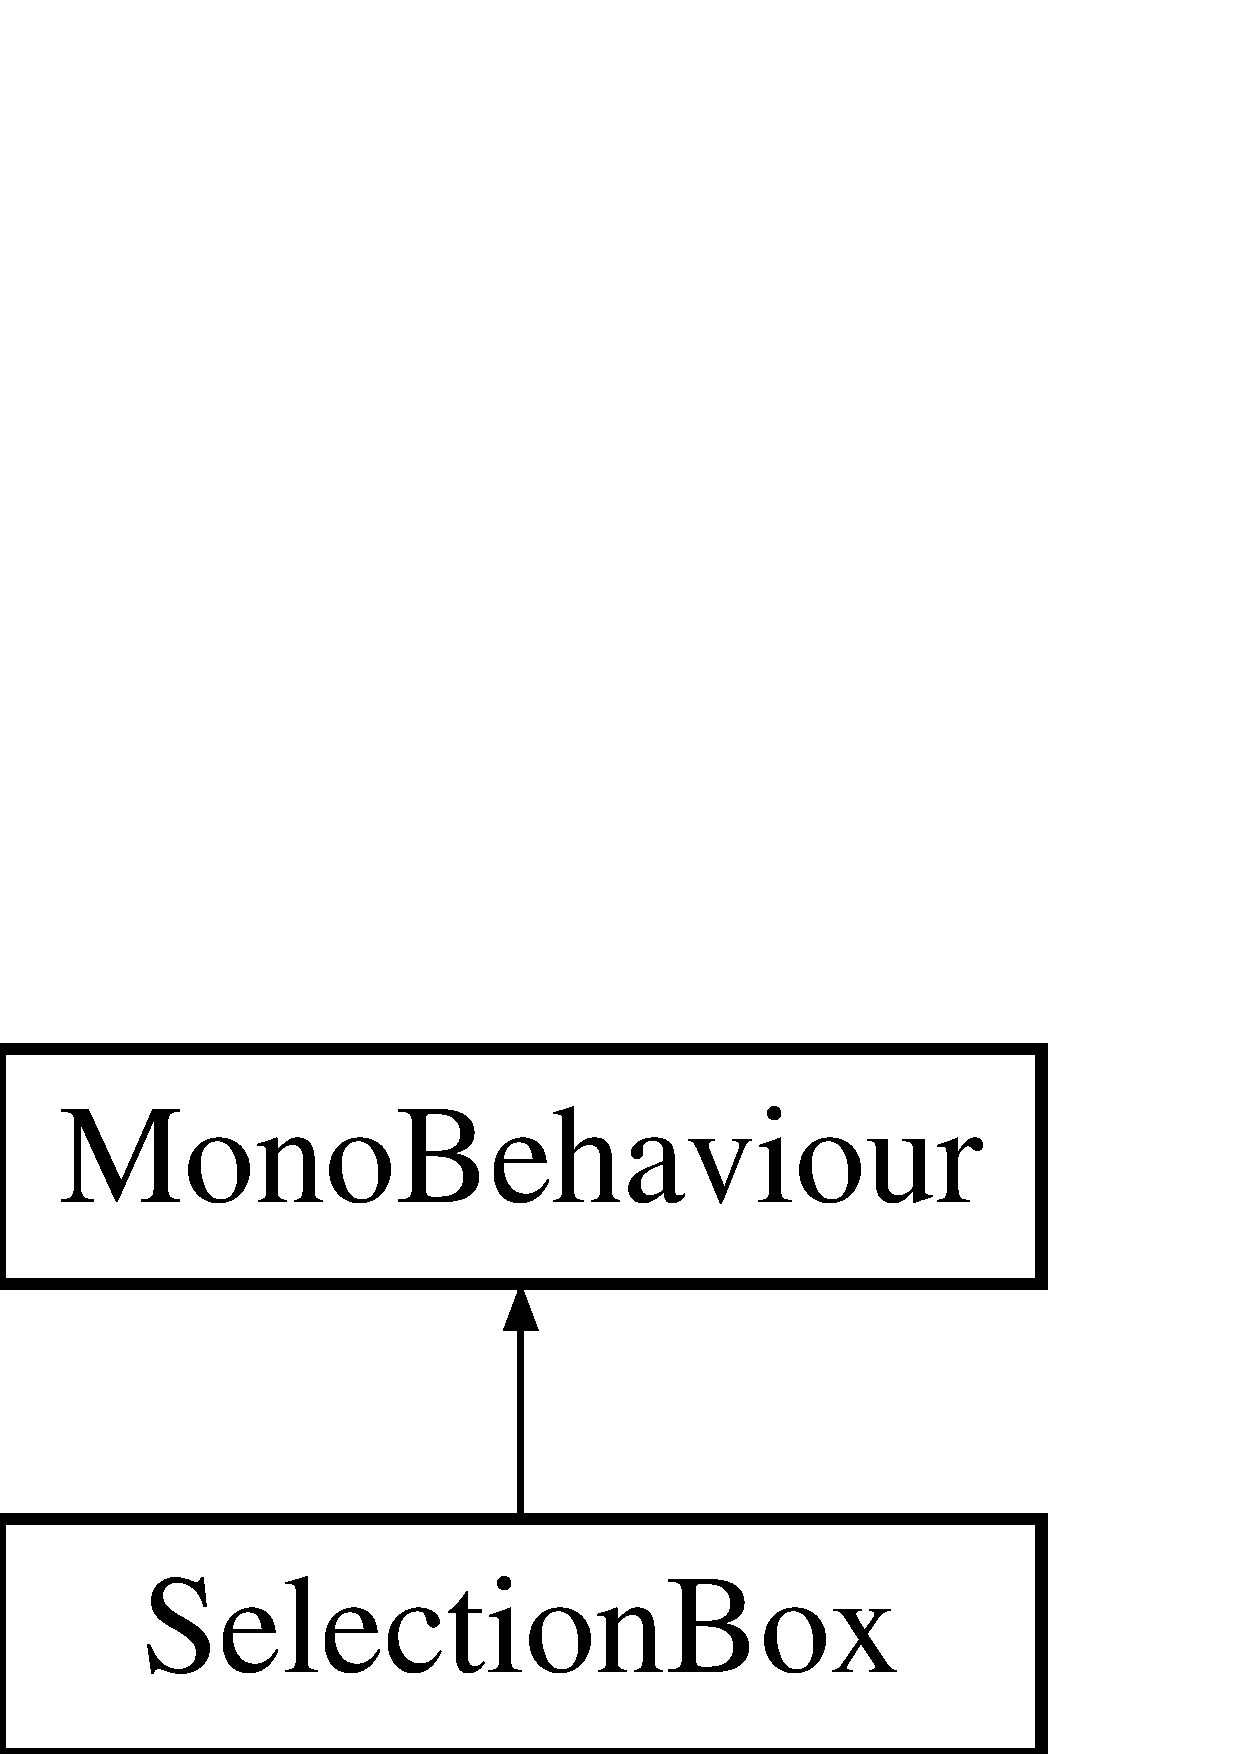
\includegraphics[height=2.000000cm]{class_selection_box}
\end{center}
\end{figure}
\subsection*{Fonctions membres publiques}
\begin{DoxyCompactItemize}
\item 
\mbox{\Hypertarget{class_selection_box_a008531028a56f9b784d05ff1fef02991}\label{class_selection_box_a008531028a56f9b784d05ff1fef02991}} 
void {\bfseries set\+Active} (bool active)
\item 
\mbox{\Hypertarget{class_selection_box_a03257767fe70c02ebb259ec80ccfd9f6}\label{class_selection_box_a03257767fe70c02ebb259ec80ccfd9f6}} 
void {\bfseries set\+Active\+When\+Realease} (bool active)
\end{DoxyCompactItemize}
\subsection*{Attributs publics}
\begin{DoxyCompactItemize}
\item 
\mbox{\Hypertarget{class_selection_box_a2ce1b3bb8021803cc1229439c8cd7a0c}\label{class_selection_box_a2ce1b3bb8021803cc1229439c8cd7a0c}} 
G\+U\+I\+Style {\bfseries select\+Texture}
\end{DoxyCompactItemize}


La documentation de cette classe a été générée à partir du fichier suivant \+:\begin{DoxyCompactItemize}
\item 
Interface/Selection\+Box.\+cs\end{DoxyCompactItemize}

\hypertarget{class_targeting_move}{}\section{Référence de la classe Targeting\+Move}
\label{class_targeting_move}\index{Targeting\+Move@{Targeting\+Move}}
Graphe d\textquotesingle{}héritage de Targeting\+Move\+:\begin{figure}[H]
\begin{center}
\leavevmode
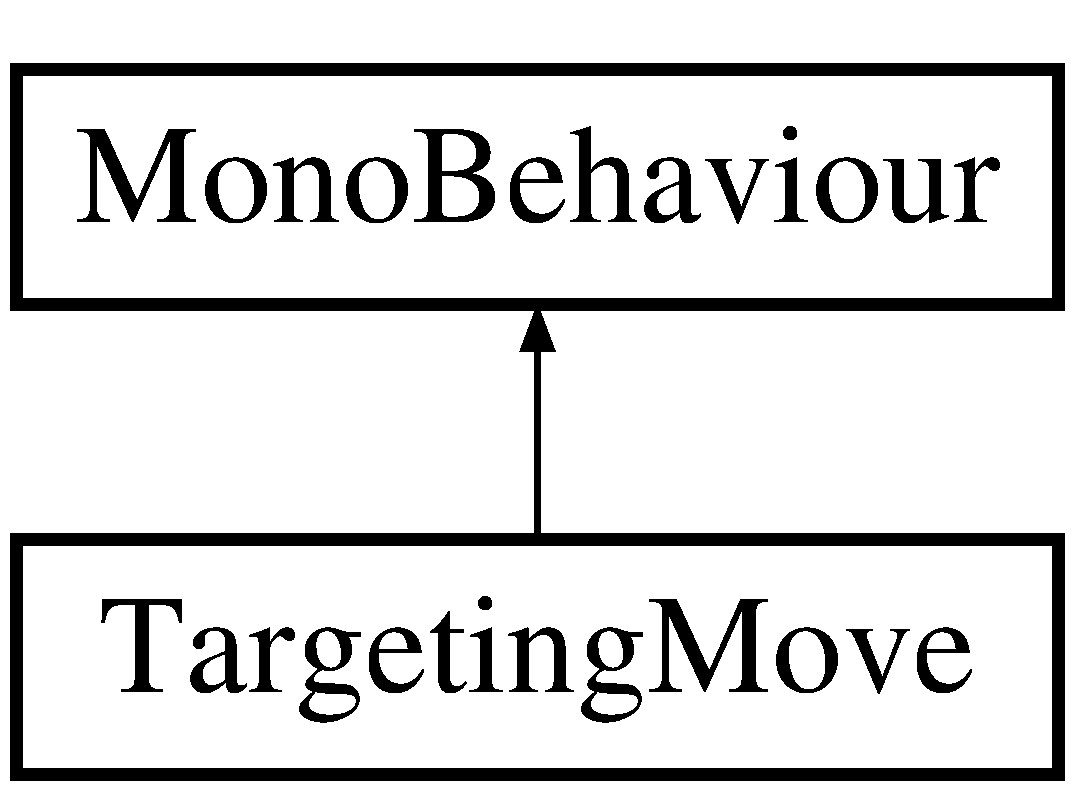
\includegraphics[height=2.000000cm]{class_targeting_move}
\end{center}
\end{figure}
\subsection*{Fonctions membres publiques}
\begin{DoxyCompactItemize}
\item 
\mbox{\Hypertarget{class_targeting_move_a65a4d699d9637b9a3aa4fcd7ee8ea4be}\label{class_targeting_move_a65a4d699d9637b9a3aa4fcd7ee8ea4be}} 
float {\bfseries round} (float a)
\end{DoxyCompactItemize}
\subsection*{Attributs publics}
\begin{DoxyCompactItemize}
\item 
float \hyperlink{class_targeting_move_a18c74fa8724c7faec50dae67ad7b527d}{speed} = 1.\+0f
\begin{DoxyCompactList}\small\item\em Vitesse de mouvement \end{DoxyCompactList}\item 
float \hyperlink{class_targeting_move_ae3c99569094a8163b09a9b9f3607e2c1}{blocksize} = 0.\+24f
\begin{DoxyCompactList}\small\item\em Taille d\textquotesingle{}un block -\/$>$ Le Pas pour un mouvement \end{DoxyCompactList}\item 
string \hyperlink{class_targeting_move_a3f08aa20c9b9db6b215d8b83113c888d}{first\+Direction} = \char`\"{}aucune\char`\"{}
\begin{DoxyCompactList}\small\item\em Direction en chaines de caractères \end{DoxyCompactList}\end{DoxyCompactItemize}
\subsection*{Attributs protégés}
\begin{DoxyCompactItemize}
\item 
\mbox{\Hypertarget{class_targeting_move_a9ed5ff56ed4f6b6cf1cd133e570d2ef3}\label{class_targeting_move_a9ed5ff56ed4f6b6cf1cd133e570d2ef3}} 
bool {\bfseries can\+Move\+Up}
\item 
\mbox{\Hypertarget{class_targeting_move_a049058e26751a97d08a808613260c66a}\label{class_targeting_move_a049058e26751a97d08a808613260c66a}} 
bool {\bfseries can\+Move\+Down}
\item 
\mbox{\Hypertarget{class_targeting_move_a7cda299d69eb179eeb89739eccb666cd}\label{class_targeting_move_a7cda299d69eb179eeb89739eccb666cd}} 
bool {\bfseries can\+Move\+Left}
\item 
\mbox{\Hypertarget{class_targeting_move_a9ddc3ed6156e8a0ef1f02400a88c66bf}\label{class_targeting_move_a9ddc3ed6156e8a0ef1f02400a88c66bf}} 
bool {\bfseries can\+Move\+Right}
\end{DoxyCompactItemize}


\subsection{Documentation des données membres}
\mbox{\Hypertarget{class_targeting_move_ae3c99569094a8163b09a9b9f3607e2c1}\label{class_targeting_move_ae3c99569094a8163b09a9b9f3607e2c1}} 
\index{Targeting\+Move@{Targeting\+Move}!blocksize@{blocksize}}
\index{blocksize@{blocksize}!Targeting\+Move@{Targeting\+Move}}
\subsubsection{\texorpdfstring{blocksize}{blocksize}}
{\footnotesize\ttfamily float Targeting\+Move.\+blocksize = 0.\+24f}



Taille d\textquotesingle{}un block -\/$>$ Le Pas pour un mouvement 

\mbox{\Hypertarget{class_targeting_move_a3f08aa20c9b9db6b215d8b83113c888d}\label{class_targeting_move_a3f08aa20c9b9db6b215d8b83113c888d}} 
\index{Targeting\+Move@{Targeting\+Move}!first\+Direction@{first\+Direction}}
\index{first\+Direction@{first\+Direction}!Targeting\+Move@{Targeting\+Move}}
\subsubsection{\texorpdfstring{first\+Direction}{firstDirection}}
{\footnotesize\ttfamily string Targeting\+Move.\+first\+Direction = \char`\"{}aucune\char`\"{}}



Direction en chaines de caractères 

\mbox{\Hypertarget{class_targeting_move_a18c74fa8724c7faec50dae67ad7b527d}\label{class_targeting_move_a18c74fa8724c7faec50dae67ad7b527d}} 
\index{Targeting\+Move@{Targeting\+Move}!speed@{speed}}
\index{speed@{speed}!Targeting\+Move@{Targeting\+Move}}
\subsubsection{\texorpdfstring{speed}{speed}}
{\footnotesize\ttfamily float Targeting\+Move.\+speed = 1.\+0f}



Vitesse de mouvement 



La documentation de cette classe a été générée à partir du fichier suivant \+:\begin{DoxyCompactItemize}
\item 
Move/Targeting\+Move.\+cs\end{DoxyCompactItemize}

\hypertarget{class_tile}{}\section{Référence de la classe Tile}
\label{class_tile}\index{Tile@{Tile}}
Graphe d\textquotesingle{}héritage de Tile\+:\begin{figure}[H]
\begin{center}
\leavevmode
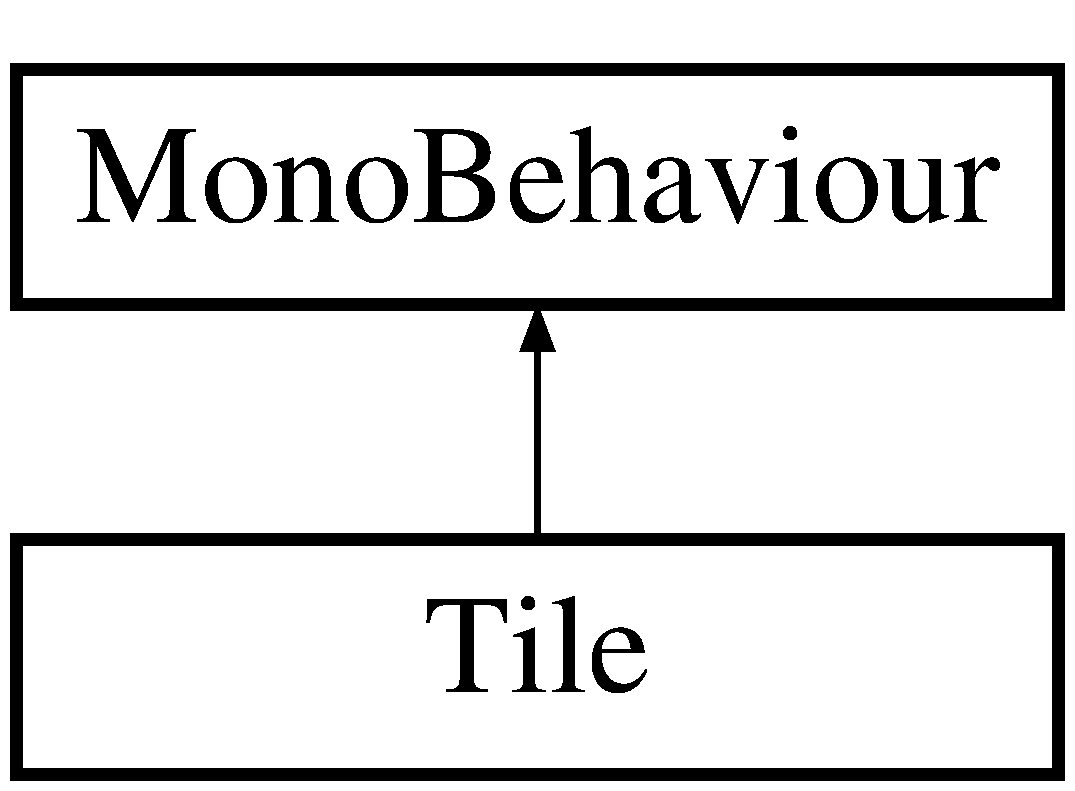
\includegraphics[height=2.000000cm]{class_tile}
\end{center}
\end{figure}
\subsection*{Fonctions membres publiques}
\begin{DoxyCompactItemize}
\item 
\mbox{\Hypertarget{class_tile_a60ee8f081cb0f74d6587a5cefc7978ba}\label{class_tile_a60ee8f081cb0f74d6587a5cefc7978ba}} 
void {\bfseries move} (int x, int y)
\end{DoxyCompactItemize}
\subsection*{Attributs publics}
\begin{DoxyCompactItemize}
\item 
\mbox{\Hypertarget{class_tile_a19beb0bc38c9fe2c8010e383f837f399}\label{class_tile_a19beb0bc38c9fe2c8010e383f837f399}} 
int {\bfseries code}
\item 
\mbox{\Hypertarget{class_tile_ad3c0cca342774de090545a0a05e5b3af}\label{class_tile_ad3c0cca342774de090545a0a05e5b3af}} 
int {\bfseries i}
\item 
\mbox{\Hypertarget{class_tile_a1a90025da8043aed9138767589671bfa}\label{class_tile_a1a90025da8043aed9138767589671bfa}} 
int {\bfseries j}
\end{DoxyCompactItemize}


La documentation de cette classe a été générée à partir du fichier suivant \+:\begin{DoxyCompactItemize}
\item 
Tile\+Map/Tile.\+cs\end{DoxyCompactItemize}

\hypertarget{class_tile_editor}{}\section{Référence de la classe Tile\+Editor}
\label{class_tile_editor}\index{Tile\+Editor@{Tile\+Editor}}
Graphe d\textquotesingle{}héritage de Tile\+Editor\+:\begin{figure}[H]
\begin{center}
\leavevmode
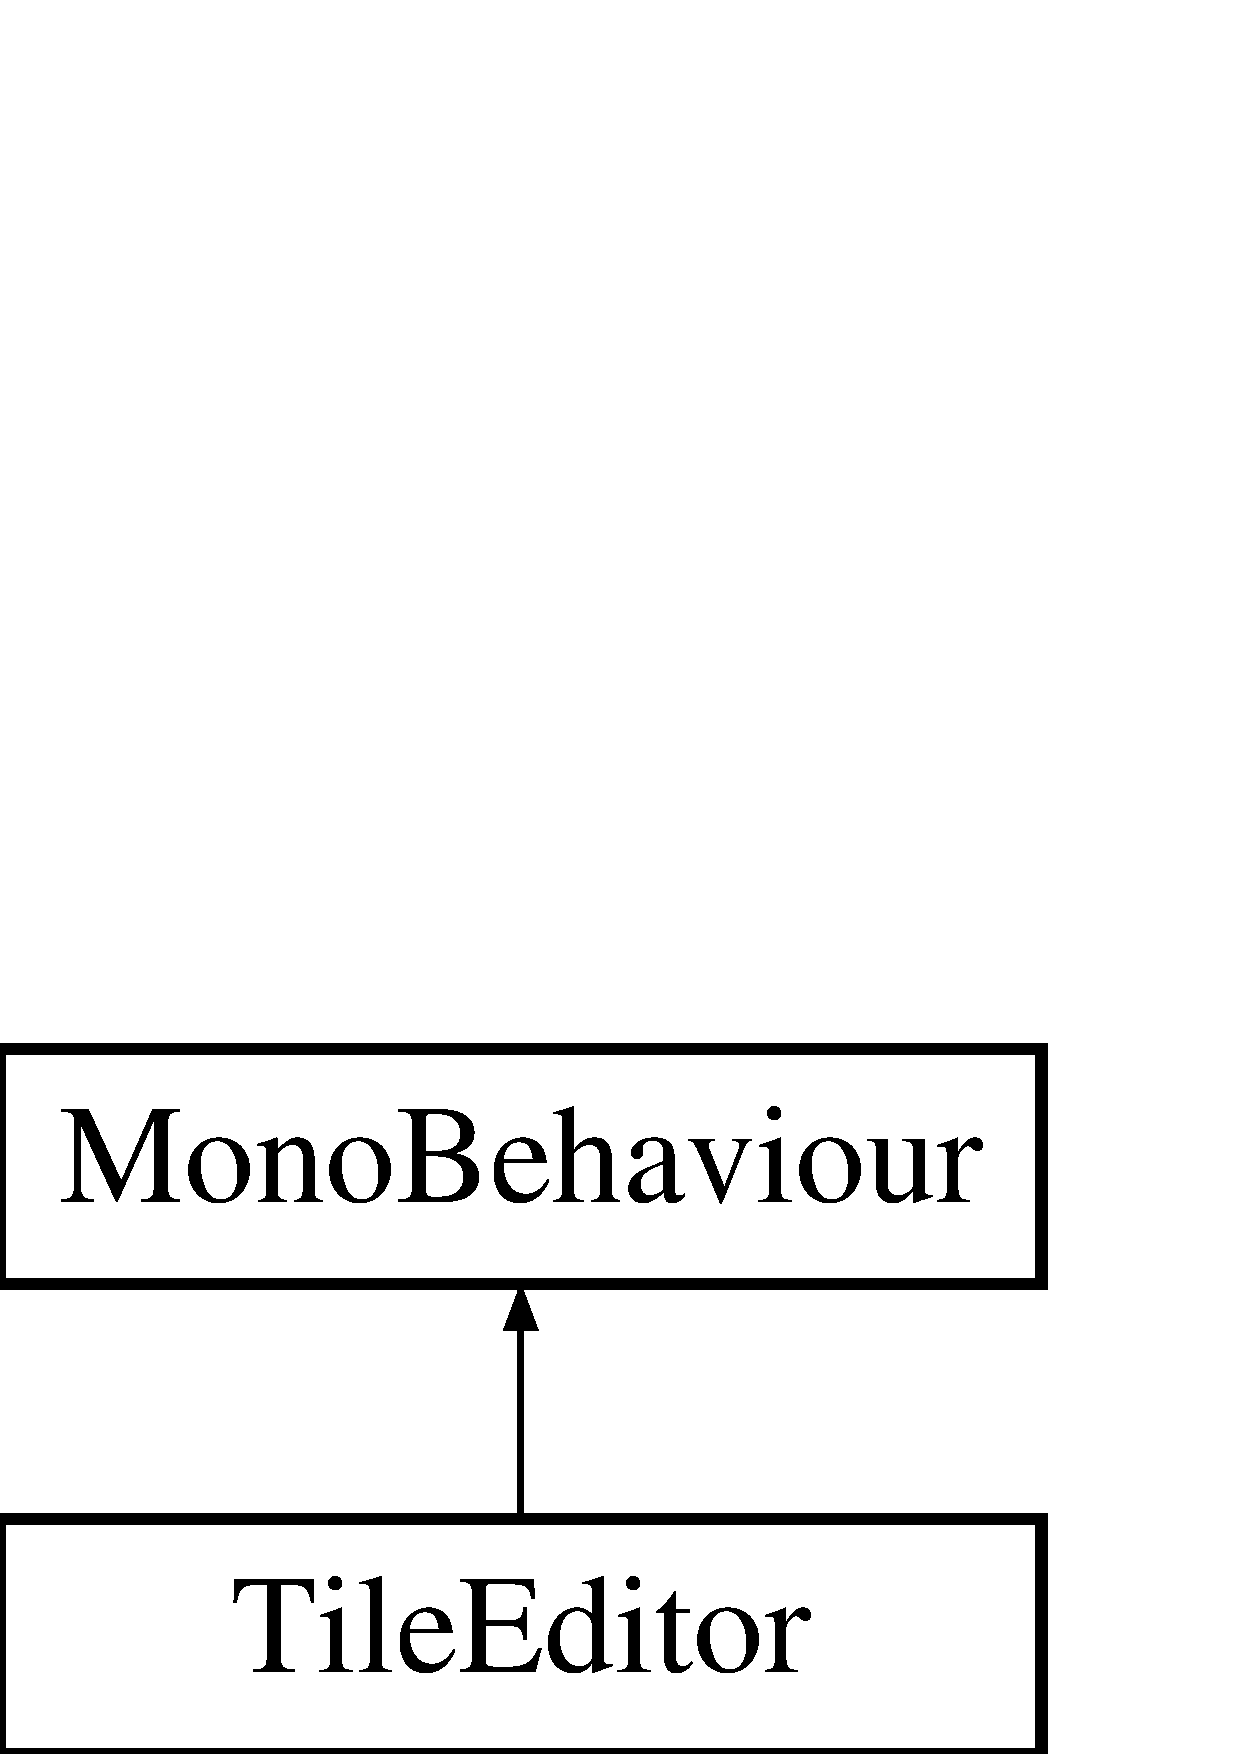
\includegraphics[height=2.000000cm]{class_tile_editor}
\end{center}
\end{figure}
\subsection*{Fonctions membres publiques}
\begin{DoxyCompactItemize}
\item 
\mbox{\Hypertarget{class_tile_editor_a388e1191821f07e9486e26ac5dd43dac}\label{class_tile_editor_a388e1191821f07e9486e26ac5dd43dac}} 
void {\bfseries Update\+Text} ()
\item 
\mbox{\Hypertarget{class_tile_editor_aac23f708649956dad2a2d143482325c4}\label{class_tile_editor_aac23f708649956dad2a2d143482325c4}} 
void {\bfseries Center\+Camera} ()
\item 
\mbox{\Hypertarget{class_tile_editor_a6e21963247a98b316944a7f184156fc6}\label{class_tile_editor_a6e21963247a98b316944a7f184156fc6}} 
void {\bfseries init\+Cursor} ()
\item 
\mbox{\Hypertarget{class_tile_editor_a4cc6ee8cc3ebf875763b9ea172910b2d}\label{class_tile_editor_a4cc6ee8cc3ebf875763b9ea172910b2d}} 
void {\bfseries create\+New\+Map} ()
\item 
\mbox{\Hypertarget{class_tile_editor_a5a9a1b757f4f2729bef6551de496dbce}\label{class_tile_editor_a5a9a1b757f4f2729bef6551de496dbce}} 
void {\bfseries tool\+Manager} ()
\item 
\mbox{\Hypertarget{class_tile_editor_aa864605629d3be9ff0fe064ed0214de1}\label{class_tile_editor_aa864605629d3be9ff0fe064ed0214de1}} 
void {\bfseries rotate\+Tile} ()
\item 
\mbox{\Hypertarget{class_tile_editor_a249e6046f5ffa05e1d38c3e7323cb5ba}\label{class_tile_editor_a249e6046f5ffa05e1d38c3e7323cb5ba}} 
void {\bfseries save\+Lvl} (string map\+Name)
\item 
\mbox{\Hypertarget{class_tile_editor_a4b65f9f7c78f28b24ce397bec4b0c5cb}\label{class_tile_editor_a4b65f9f7c78f28b24ce397bec4b0c5cb}} 
void {\bfseries load\+Lvl} (string map\+Name)
\item 
\mbox{\Hypertarget{class_tile_editor_a187c8ed997a91cd17b4179b1ae836964}\label{class_tile_editor_a187c8ed997a91cd17b4179b1ae836964}} 
void {\bfseries play\+Lvl} ()
\item 
\mbox{\Hypertarget{class_tile_editor_a90f35fb468749184ebab36e3aa3efc2f}\label{class_tile_editor_a90f35fb468749184ebab36e3aa3efc2f}} 
void {\bfseries Add\+Line} ()
\item 
\mbox{\Hypertarget{class_tile_editor_af516c78b0d4d5241f681fe0aa90cd8b1}\label{class_tile_editor_af516c78b0d4d5241f681fe0aa90cd8b1}} 
void {\bfseries Remove\+Row} ()
\item 
\mbox{\Hypertarget{class_tile_editor_a77c85603abe7abfb74988c113ee66d1b}\label{class_tile_editor_a77c85603abe7abfb74988c113ee66d1b}} 
void {\bfseries Add\+Column} ()
\item 
\mbox{\Hypertarget{class_tile_editor_a918419a21cbf0897792728d0e85a2658}\label{class_tile_editor_a918419a21cbf0897792728d0e85a2658}} 
void {\bfseries Remove\+Column} ()
\item 
\mbox{\Hypertarget{class_tile_editor_a9e661ae8f6019b0ca6ca3772147c335c}\label{class_tile_editor_a9e661ae8f6019b0ca6ca3772147c335c}} 
void {\bfseries toggle\+Mono\+Tile\+Tool} ()
\item 
\mbox{\Hypertarget{class_tile_editor_aa877586ba870a10be5a6946d115e915e}\label{class_tile_editor_aa877586ba870a10be5a6946d115e915e}} 
void {\bfseries toggle\+Draw\+Rect\+Full\+Tool} ()
\item 
\mbox{\Hypertarget{class_tile_editor_a0b3d832aca0a89a447c6c6cfe3baf96c}\label{class_tile_editor_a0b3d832aca0a89a447c6c6cfe3baf96c}} 
void {\bfseries toggle\+Draw\+Rect\+Corner\+Tool} ()
\item 
\mbox{\Hypertarget{class_tile_editor_a51f70c01956b2207659b746d378ce0f8}\label{class_tile_editor_a51f70c01956b2207659b746d378ce0f8}} 
void {\bfseries toggle\+Copy\+Selector} ()
\item 
\mbox{\Hypertarget{class_tile_editor_aa6cdbe7245898a8eda694f516564d66a}\label{class_tile_editor_aa6cdbe7245898a8eda694f516564d66a}} 
void {\bfseries Select\+Empty} ()
\item 
\mbox{\Hypertarget{class_tile_editor_ad915164eb968f728101a78110aa3bcc9}\label{class_tile_editor_ad915164eb968f728101a78110aa3bcc9}} 
void {\bfseries Select\+Angle1} ()
\item 
\mbox{\Hypertarget{class_tile_editor_aeaeffd5fe7884a315fa96feeea8f08df}\label{class_tile_editor_aeaeffd5fe7884a315fa96feeea8f08df}} 
void {\bfseries Select\+Angle2} ()
\item 
\mbox{\Hypertarget{class_tile_editor_a79a169abac2010e0715f8a1a251de457}\label{class_tile_editor_a79a169abac2010e0715f8a1a251de457}} 
void {\bfseries Select\+Angle3} ()
\item 
\mbox{\Hypertarget{class_tile_editor_a63986469ed1932c42ddff7c27fd307eb}\label{class_tile_editor_a63986469ed1932c42ddff7c27fd307eb}} 
void {\bfseries Select\+Angle4} ()
\item 
\mbox{\Hypertarget{class_tile_editor_a461fe707bd7ae7ea2e0b64f5e4698d7a}\label{class_tile_editor_a461fe707bd7ae7ea2e0b64f5e4698d7a}} 
void {\bfseries Select\+Mur1} ()
\item 
\mbox{\Hypertarget{class_tile_editor_a1a1095fba5c80cfaa7321661b17a8205}\label{class_tile_editor_a1a1095fba5c80cfaa7321661b17a8205}} 
void {\bfseries Select\+Mur2} ()
\item 
\mbox{\Hypertarget{class_tile_editor_aa8e912179bca72c33d1bd14a088140fb}\label{class_tile_editor_aa8e912179bca72c33d1bd14a088140fb}} 
void {\bfseries Select\+Mur3} ()
\item 
\mbox{\Hypertarget{class_tile_editor_a32ea15832c9c8c1617ffebdf1cf60057}\label{class_tile_editor_a32ea15832c9c8c1617ffebdf1cf60057}} 
void {\bfseries Select\+Block1} ()
\item 
\mbox{\Hypertarget{class_tile_editor_a332ee4658213072d8e5ff5f3d37703f1}\label{class_tile_editor_a332ee4658213072d8e5ff5f3d37703f1}} 
void {\bfseries Select\+Block2} ()
\item 
\mbox{\Hypertarget{class_tile_editor_a66d074b9d46aeea6dc74603779733bb9}\label{class_tile_editor_a66d074b9d46aeea6dc74603779733bb9}} 
void {\bfseries Select\+Block3} ()
\item 
\mbox{\Hypertarget{class_tile_editor_a00e6d6c76670fa163a5aba688fdd3a35}\label{class_tile_editor_a00e6d6c76670fa163a5aba688fdd3a35}} 
void {\bfseries Select\+Pacman} ()
\item 
\mbox{\Hypertarget{class_tile_editor_a1a6cac1d7528055ba5b4fa5a086b2cd8}\label{class_tile_editor_a1a6cac1d7528055ba5b4fa5a086b2cd8}} 
void {\bfseries Select\+Blinky} ()
\item 
\mbox{\Hypertarget{class_tile_editor_a95b6903481e5583bdee91f67ad08b4e5}\label{class_tile_editor_a95b6903481e5583bdee91f67ad08b4e5}} 
void {\bfseries Select\+Inky} ()
\item 
\mbox{\Hypertarget{class_tile_editor_a248d8c0a237675a1648c611dd788ce07}\label{class_tile_editor_a248d8c0a237675a1648c611dd788ce07}} 
void {\bfseries Select\+Pinky} ()
\item 
\mbox{\Hypertarget{class_tile_editor_a69c0b077eed85424478e7cb7f14041cc}\label{class_tile_editor_a69c0b077eed85424478e7cb7f14041cc}} 
void {\bfseries Select\+Clyde} ()
\item 
\mbox{\Hypertarget{class_tile_editor_ad884bfd125f75bd2d8c659377086a16d}\label{class_tile_editor_ad884bfd125f75bd2d8c659377086a16d}} 
void {\bfseries Select\+Power1} ()
\item 
\mbox{\Hypertarget{class_tile_editor_a58cee2ae8581633cb57b5caa77938ead}\label{class_tile_editor_a58cee2ae8581633cb57b5caa77938ead}} 
void {\bfseries Select\+Bonus} ()
\item 
\mbox{\Hypertarget{class_tile_editor_a52056ce8c5cf8d6b4a518b610889b1e4}\label{class_tile_editor_a52056ce8c5cf8d6b4a518b610889b1e4}} 
void {\bfseries Select\+Porte} ()
\end{DoxyCompactItemize}
\subsection*{Attributs publics}
\begin{DoxyCompactItemize}
\item 
\mbox{\Hypertarget{class_tile_editor_ad67ea049f4485bcf8cedaed0b91b8f27}\label{class_tile_editor_ad67ea049f4485bcf8cedaed0b91b8f27}} 
int {\bfseries hauteur}
\item 
\mbox{\Hypertarget{class_tile_editor_a0a7aa087db46467b48265d136d7c4aa9}\label{class_tile_editor_a0a7aa087db46467b48265d136d7c4aa9}} 
int {\bfseries largeur}
\item 
\mbox{\Hypertarget{class_tile_editor_a9d6224f7e21a59de68e7d16c3379a699}\label{class_tile_editor_a9d6224f7e21a59de68e7d16c3379a699}} 
Text {\bfseries nb\+Colonnes}
\item 
\mbox{\Hypertarget{class_tile_editor_a1f11f4caa9713463fe1a489d45c1f88b}\label{class_tile_editor_a1f11f4caa9713463fe1a489d45c1f88b}} 
Text {\bfseries nb\+Lignes}
\item 
\mbox{\Hypertarget{class_tile_editor_a911d69f085dfd546c7c14c613e4602c6}\label{class_tile_editor_a911d69f085dfd546c7c14c613e4602c6}} 
float {\bfseries move\+Speed} = 1.\+0f
\end{DoxyCompactItemize}
\subsection*{Attributs protégés}
\begin{DoxyCompactItemize}
\item 
\mbox{\Hypertarget{class_tile_editor_ac1ba22e5c189adf64f6eb71ed90d5924}\label{class_tile_editor_ac1ba22e5c189adf64f6eb71ed90d5924}} 
\hyperlink{class_tile_matrix}{Tile\+Matrix} {\bfseries tile\+Mat}
\item 
\mbox{\Hypertarget{class_tile_editor_a222606c81c49c52b69eadb80103484ff}\label{class_tile_editor_a222606c81c49c52b69eadb80103484ff}} 
string {\bfseries tiles\+Path} = \char`\"{}Sprites/Default/tiles\char`\"{}
\item 
\mbox{\Hypertarget{class_tile_editor_a2ca856979ced0f783d77d0fe80a16cf8}\label{class_tile_editor_a2ca856979ced0f783d77d0fe80a16cf8}} 
bool {\bfseries is\+Playing} = false
\item 
\mbox{\Hypertarget{class_tile_editor_a48d125806d896759d59983afc8aa345b}\label{class_tile_editor_a48d125806d896759d59983afc8aa345b}} 
bool {\bfseries allow\+Mouse\+Interaction} = true
\item 
int \hyperlink{class_tile_editor_a6b7e8a9c28da445fcc357c5814ec2c7e}{sprite\+Val\+On\+Click} = 1
\begin{DoxyCompactList}\small\item\em selection et rotation tiles \end{DoxyCompactList}\item 
\mbox{\Hypertarget{class_tile_editor_a30265310bbb8b7e488c4ff7e50420d07}\label{class_tile_editor_a30265310bbb8b7e488c4ff7e50420d07}} 
int {\bfseries selected\+Tile} = 1
\item 
\mbox{\Hypertarget{class_tile_editor_ac336b90b7a83a77ba980ddf5cda8b47c}\label{class_tile_editor_ac336b90b7a83a77ba980ddf5cda8b47c}} 
bool {\bfseries rotation360} = true
\item 
\mbox{\Hypertarget{class_tile_editor_a2470a66145457aa97b863f3e055f61ff}\label{class_tile_editor_a2470a66145457aa97b863f3e055f61ff}} 
bool {\bfseries rotation90} = false
\item 
\mbox{\Hypertarget{class_tile_editor_ab73669828f4e63cf8fd9de53fb51d88a}\label{class_tile_editor_ab73669828f4e63cf8fd9de53fb51d88a}} 
int {\bfseries nb\+Rotation} = 0
\item 
\mbox{\Hypertarget{class_tile_editor_ac80e6143a31707c94eccd73b13d66094}\label{class_tile_editor_ac80e6143a31707c94eccd73b13d66094}} 
bool {\bfseries drag} = false
\item 
\mbox{\Hypertarget{class_tile_editor_ae0ba64039ce6bf8747c164c666e714e6}\label{class_tile_editor_ae0ba64039ce6bf8747c164c666e714e6}} 
bool {\bfseries rectangular\+Selection} = false
\item 
\mbox{\Hypertarget{class_tile_editor_af8c66222b14bf34c702809e39a94f17d}\label{class_tile_editor_af8c66222b14bf34c702809e39a94f17d}} 
bool {\bfseries rect\+Full}
\item 
\mbox{\Hypertarget{class_tile_editor_a2f5d208f98e7ebb1cae7c3ac6f349e2f}\label{class_tile_editor_a2f5d208f98e7ebb1cae7c3ac6f349e2f}} 
bool {\bfseries rect\+Corner}
\item 
\mbox{\Hypertarget{class_tile_editor_a6830d0ecc636bb141679785f3e3713ed}\label{class_tile_editor_a6830d0ecc636bb141679785f3e3713ed}} 
bool {\bfseries rect\+Copy}
\item 
\mbox{\Hypertarget{class_tile_editor_a365f6f86094835272a448764b9419653}\label{class_tile_editor_a365f6f86094835272a448764b9419653}} 
bool {\bfseries copy\+Rect\+Is\+Set}
\item 
\mbox{\Hypertarget{class_tile_editor_a19a8de643670bf211a16feb3a9e0de3d}\label{class_tile_editor_a19a8de643670bf211a16feb3a9e0de3d}} 
int {\bfseries I\+On\+Click} = -\/1
\item 
\mbox{\Hypertarget{class_tile_editor_a35658cbe4ac32fdf551c23117260569e}\label{class_tile_editor_a35658cbe4ac32fdf551c23117260569e}} 
int {\bfseries J\+On\+Click} = -\/1
\item 
\mbox{\Hypertarget{class_tile_editor_a23bd906c713e4dfa02307b646cc6a2f2}\label{class_tile_editor_a23bd906c713e4dfa02307b646cc6a2f2}} 
int {\bfseries I\+On\+Release} = -\/1
\item 
\mbox{\Hypertarget{class_tile_editor_a785ea604015e670cfa9077a4d654de64}\label{class_tile_editor_a785ea604015e670cfa9077a4d654de64}} 
int {\bfseries J\+On\+Release} = -\/1
\item 
\mbox{\Hypertarget{class_tile_editor_aa3ef0a115002c133e311f3fee9afc9ae}\label{class_tile_editor_aa3ef0a115002c133e311f3fee9afc9ae}} 
int {\bfseries I\+Min} = -\/1
\item 
\mbox{\Hypertarget{class_tile_editor_afee9b8631e503c1cb7fdcae917f92dd6}\label{class_tile_editor_afee9b8631e503c1cb7fdcae917f92dd6}} 
int {\bfseries J\+Min} = -\/1
\item 
\mbox{\Hypertarget{class_tile_editor_afba62d18bc3e84b4afd1b5249bc1f86d}\label{class_tile_editor_afba62d18bc3e84b4afd1b5249bc1f86d}} 
int {\bfseries I\+Max} = -\/1
\item 
\mbox{\Hypertarget{class_tile_editor_a6d4a70954ddad9468e0fb4824587960c}\label{class_tile_editor_a6d4a70954ddad9468e0fb4824587960c}} 
int {\bfseries J\+Max} = -\/1
\item 
\mbox{\Hypertarget{class_tile_editor_ab880b414b6ae4a4eec0a74a8464fd74f}\label{class_tile_editor_ab880b414b6ae4a4eec0a74a8464fd74f}} 
List$<$ int $>$ {\bfseries copy\+Rect\+Buffer} = null
\item 
\mbox{\Hypertarget{class_tile_editor_aa67963a2d122ecdd3ecb591dd28c8856}\label{class_tile_editor_aa67963a2d122ecdd3ecb591dd28c8856}} 
float {\bfseries Camera\+Init\+Size}
\item 
\mbox{\Hypertarget{class_tile_editor_a29e537a4bffe84702bb7ba5c6788f890}\label{class_tile_editor_a29e537a4bffe84702bb7ba5c6788f890}} 
Vector3 {\bfseries Camera\+Init\+Pos}
\item 
Game\+Object \hyperlink{class_tile_editor_a7419b8c1c2c27a10a82767f7667f3d8b}{cursor\+Sprite}
\begin{DoxyCompactList}\small\item\em gestion curseur souris \end{DoxyCompactList}\end{DoxyCompactItemize}


\subsection{Documentation des données membres}
\mbox{\Hypertarget{class_tile_editor_a7419b8c1c2c27a10a82767f7667f3d8b}\label{class_tile_editor_a7419b8c1c2c27a10a82767f7667f3d8b}} 
\index{Tile\+Editor@{Tile\+Editor}!cursor\+Sprite@{cursor\+Sprite}}
\index{cursor\+Sprite@{cursor\+Sprite}!Tile\+Editor@{Tile\+Editor}}
\subsubsection{\texorpdfstring{cursor\+Sprite}{cursorSprite}}
{\footnotesize\ttfamily Game\+Object Tile\+Editor.\+cursor\+Sprite\hspace{0.3cm}{\ttfamily [protected]}}



gestion curseur souris 

\mbox{\Hypertarget{class_tile_editor_a6b7e8a9c28da445fcc357c5814ec2c7e}\label{class_tile_editor_a6b7e8a9c28da445fcc357c5814ec2c7e}} 
\index{Tile\+Editor@{Tile\+Editor}!sprite\+Val\+On\+Click@{sprite\+Val\+On\+Click}}
\index{sprite\+Val\+On\+Click@{sprite\+Val\+On\+Click}!Tile\+Editor@{Tile\+Editor}}
\subsubsection{\texorpdfstring{sprite\+Val\+On\+Click}{spriteValOnClick}}
{\footnotesize\ttfamily int Tile\+Editor.\+sprite\+Val\+On\+Click = 1\hspace{0.3cm}{\ttfamily [protected]}}



selection et rotation tiles 



La documentation de cette classe a été générée à partir du fichier suivant \+:\begin{DoxyCompactItemize}
\item 
Tile\+Map/Tile\+Editor.\+cs\end{DoxyCompactItemize}

\hypertarget{class_tile_matrix}{}\section{Référence de la classe Tile\+Matrix}
\label{class_tile_matrix}\index{Tile\+Matrix@{Tile\+Matrix}}


La class \hyperlink{class_tile_matrix}{Tile\+Matrix} permet de modifier des Matrices de Tuiles ainsi que de les charger/sauvegarder dans des fichiers.  


Graphe d\textquotesingle{}héritage de Tile\+Matrix\+:\begin{figure}[H]
\begin{center}
\leavevmode
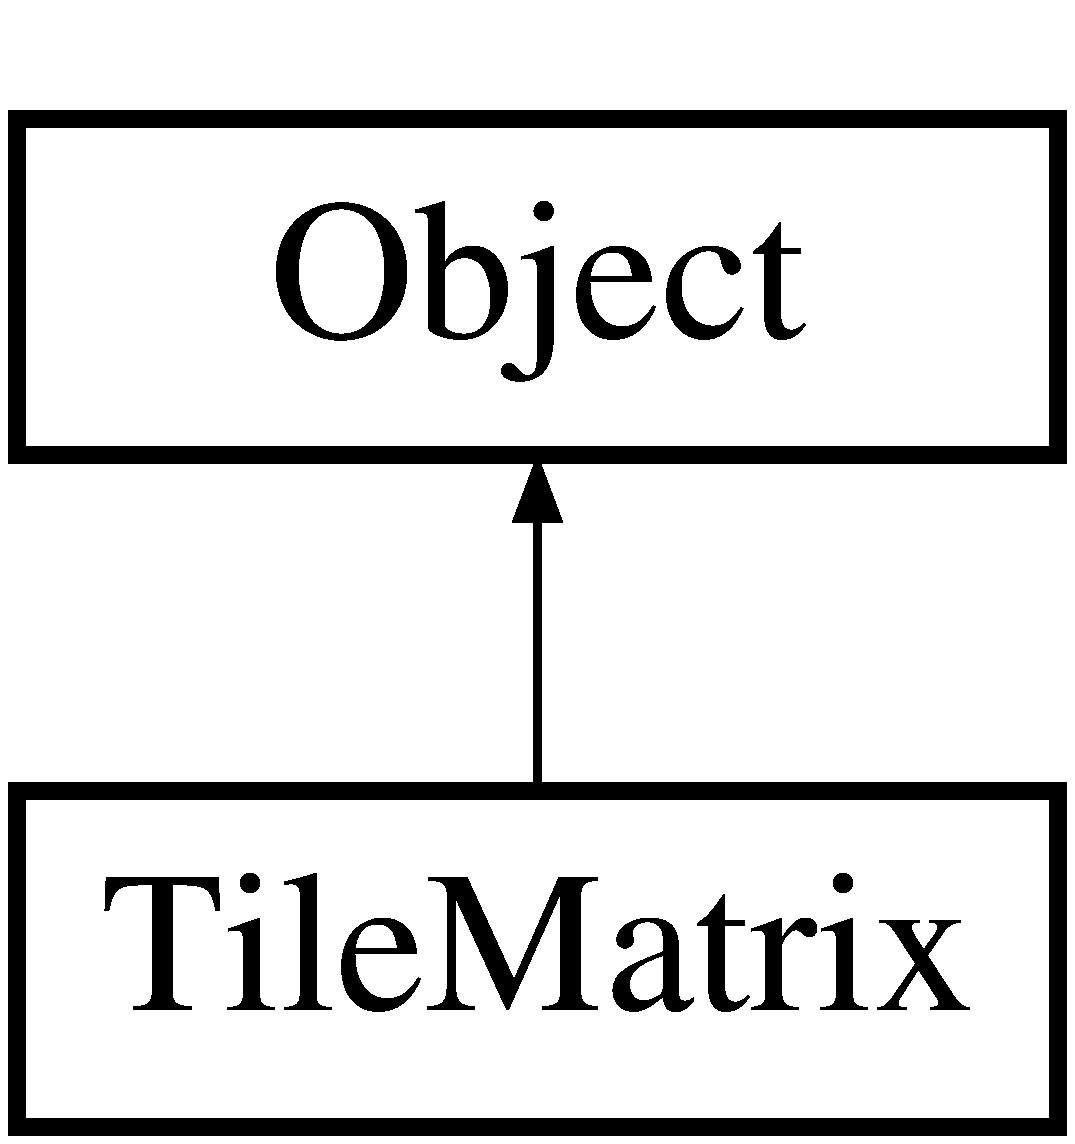
\includegraphics[height=2.000000cm]{class_tile_matrix}
\end{center}
\end{figure}
\subsection*{Fonctions membres publiques}
\begin{DoxyCompactItemize}
\item 
bool \hyperlink{class_tile_matrix_a0cdc3972eeb32776a7e1e28dc14cb0de}{is\+Empty} ()
\begin{DoxyCompactList}\small\item\em Verifie si la \hyperlink{class_tile_matrix}{Tile\+Matrix} est vide (hauteur et largeur nulle). \end{DoxyCompactList}\item 
Sprite \hyperlink{class_tile_matrix_a68d291b38ca0942fbf51683f3df2f0a6}{load\+Sprite} (int sprite\+Number)
\begin{DoxyCompactList}\small\item\em Charge un sprite à partir d\textquotesingle{}un entier envoie un message d\textquotesingle{}erreur si le l\textquotesingle{}entier est trop bas où trop grand \end{DoxyCompactList}\item 
void \hyperlink{class_tile_matrix_a093a489c26d38f24eb33caca39b6d8f7}{update\+Tile\+At} (int i, int j, int Tile\+Code)
\begin{DoxyCompactList}\small\item\em Modifie une Tuile de la \hyperlink{class_tile_matrix}{Tile\+Matrix} avec un entier qui code une Tuile. \end{DoxyCompactList}\item 
Game\+Object \hyperlink{class_tile_matrix_a8a16545b24b05b208469e9d58654b916}{Create\+Tile} (int i, int j, int num\+Sprite)
\begin{DoxyCompactList}\small\item\em Creer une Tuile à partir d\textquotesingle{}un numéro de ligne, de colonne et d\textquotesingle{}un numero corespondant à un Sprite à charger dans cette Tuile. \end{DoxyCompactList}\item 
\hyperlink{class_tile_matrix_a2fd594060764e898a105c2452d75f46f}{Tile\+Matrix} (Vector2 \hyperlink{class_tile_matrix_ac005af42acbdcf02179ba2514d20f59a}{position}, string tiles\+Path)
\begin{DoxyCompactList}\small\item\em Constructeur par default. \end{DoxyCompactList}\item 
\hyperlink{class_tile_matrix_a64f9596f9d73b577fbd3d1df5ee412a8}{Tile\+Matrix} (int \hyperlink{class_tile_matrix_a03b3e21bbee70f916ba6075150d8570b}{hauteur}, int \hyperlink{class_tile_matrix_adbffb02d3f0eba910ccbe6054a776105}{largeur}, Vector2 \hyperlink{class_tile_matrix_ac005af42acbdcf02179ba2514d20f59a}{position}, string tiles\+Path, int tile\+Number)
\begin{DoxyCompactList}\small\item\em Constructeur avec plus de paramètres. \end{DoxyCompactList}\item 
\hyperlink{class_tile_matrix_aa58cf34f960df2c3247fffce1ff53fcf}{Tile\+Matrix} (\hyperlink{class_tile_matrix}{Tile\+Matrix} M)
\begin{DoxyCompactList}\small\item\em Constructeur par copy. \end{DoxyCompactList}\item 
void \hyperlink{class_tile_matrix_a0e990be66abfae5959b5bacb8c3c25c4}{copy} (\hyperlink{class_tile_matrix}{Tile\+Matrix} M)
\begin{DoxyCompactList}\small\item\em Copie toute les valeur et le format d\textquotesingle{}une \hyperlink{class_matrice}{Matrice} M. \end{DoxyCompactList}\item 
double \hyperlink{class_tile_matrix_ab32694c884107298c3bb5fdc0f4622b3}{max} ()
\begin{DoxyCompactList}\small\item\em Max \end{DoxyCompactList}\item 
int \hyperlink{class_tile_matrix_a488170ba429dc466153ae164ed3eb5b7}{get\+Tile\+Code\+At} (int i, int j)
\begin{DoxyCompactList}\small\item\em Accesseur en lecture sur L\textquotesingle{}entier qui code la Tuile à la ligne i et la colonne j de la \hyperlink{class_tile_matrix}{Tile\+Matrix}. \end{DoxyCompactList}\item 
void \hyperlink{class_tile_matrix_aa565334932b2541174e3601bf1fcaa0a}{set\+Tile\+Code\+At} (int i, int j, int val)
\begin{DoxyCompactList}\small\item\em Modifie le code de la Tuile à la ligne i et la colonne j de la \hyperlink{class_tile_matrix}{Tile\+Matrix}. \end{DoxyCompactList}\item 
void \hyperlink{class_tile_matrix_a6b17e33f46e947e5cb81a0c056e17614}{move\+Line\+At} (int i, int stepX, int stepY)
\begin{DoxyCompactList}\small\item\em Deplace une ligne de la \hyperlink{class_tile_matrix}{Tile\+Matrix} à l\textquotesingle{}affichage. \end{DoxyCompactList}\item 
void \hyperlink{class_tile_matrix_ae524f79b278e3e77c428d33f69e82508}{move\+Colomn\+At} (int j, int stepX, int stepY)
\begin{DoxyCompactList}\small\item\em Deplace une colonne de la \hyperlink{class_tile_matrix}{Tile\+Matrix} à l\textquotesingle{}affichage. \end{DoxyCompactList}\item 
void \hyperlink{class_tile_matrix_afc71f9142da00380320980d56eef47ab}{move\+Lines\+Between} (int i1, int i2, int stepX, int stepY)
\begin{DoxyCompactList}\small\item\em Deplace certaine lignes de la \hyperlink{class_tile_matrix}{Tile\+Matrix} à l\textquotesingle{}affichage. \end{DoxyCompactList}\item 
void \hyperlink{class_tile_matrix_a3e5871c9ab9dab10f83c86584db871f7}{move\+Columns\+Between} (int j1, int j2, int stepX, int stepY)
\begin{DoxyCompactList}\small\item\em Deplace certaine colonnes de la \hyperlink{class_tile_matrix}{Tile\+Matrix} à l\textquotesingle{}affichage. \end{DoxyCompactList}\item 
void \hyperlink{class_tile_matrix_aa54a37298476381854db5a561de3fbc0}{Add\+Line} (int tile\+Number)
\begin{DoxyCompactList}\small\item\em Ajoute une ligne à la fin de la \hyperlink{class_tile_matrix}{Tile\+Matrix}. \end{DoxyCompactList}\item 
void \hyperlink{class_tile_matrix_a9ca9a8babaf656aa675af069caf90e90}{Add\+Column} (int tile\+Number)
\begin{DoxyCompactList}\small\item\em Ajoute une colonne à la fin de la \hyperlink{class_tile_matrix}{Tile\+Matrix}. \end{DoxyCompactList}\item 
void \hyperlink{class_tile_matrix_ad3dc00ccf107bf42068ed0dc2be5bc3b}{insert\+Ligne\+At} (int i, int tile\+Number)
\begin{DoxyCompactList}\small\item\em Insert une ligne dans la \hyperlink{class_tile_matrix}{Tile\+Matrix}. \end{DoxyCompactList}\item 
void \hyperlink{class_tile_matrix_a0726b04506143b1710bb87b4565d9738}{insert\+Colonne\+At} (int j, int tile\+Number)
\begin{DoxyCompactList}\small\item\em Insert une colonne dans la \hyperlink{class_matrice}{Matrice}. \end{DoxyCompactList}\item 
void \hyperlink{class_tile_matrix_ab1c633e4f9e6d6f9c3d5ffa87723ad5c}{destroy} ()
\begin{DoxyCompactList}\small\item\em Detruit entierement la \hyperlink{class_tile_matrix}{Tile\+Matrix}. \end{DoxyCompactList}\item 
void \hyperlink{class_tile_matrix_a2edc148c07d023408d1a659b8033e0f4}{remove\+Ligne\+At} (int i)
\begin{DoxyCompactList}\small\item\em Supprime une ligne de la tile\+Matrix. \end{DoxyCompactList}\item 
void \hyperlink{class_tile_matrix_a8756d0d2b534e557db1f7555f32a9ff9}{remove\+Colonne\+At} (int j)
\begin{DoxyCompactList}\small\item\em Supprime une colonne de la tile\+Matrix. \end{DoxyCompactList}\item 
void \hyperlink{class_tile_matrix_a1ff5f7a4550c1fb5214f8a2f3d585c88}{set\+Ligne} (int i, int tile\+Number)
\begin{DoxyCompactList}\small\item\em Accesseur en ecriture, change toute les Tuiles d\textquotesingle{}une ligne. \end{DoxyCompactList}\item 
void \hyperlink{class_tile_matrix_a646d11a4f74c0663bd772cf114d6fc5b}{set\+Colonne} (int j, int tile\+Number)
\begin{DoxyCompactList}\small\item\em Accesseur en ecriture, change toute les Tuiles d\textquotesingle{}une colonne. \end{DoxyCompactList}\item 
void \hyperlink{class_tile_matrix_a35a767fec694f00e38bbd04efbb5c875}{draw\+Rect\+Full} (int i\+Min, int i\+Max, int j\+Min, int j\+Max, int tile\+Code)
\begin{DoxyCompactList}\small\item\em Dessine un rectangle composé d\textquotesingle{}une certaine Tuile. \end{DoxyCompactList}\item 
void \hyperlink{class_tile_matrix_a4ec108d873c8d6aa686ecea4aa8b270b}{draw\+Rect\+Corner} (int i\+Min, int i\+Max, int j\+Min, int j\+Max, int tile\+Code)
\begin{DoxyCompactList}\small\item\em Dessine un cadre composé d\textquotesingle{}une certaine Tuile dans la \hyperlink{class_tile_matrix}{Tile\+Matrix}. \end{DoxyCompactList}\item 
List$<$ int $>$ \hyperlink{class_tile_matrix_a789263572eb4022a693fe71a6c8b5f38}{draw\+Rect\+To\+Buffer} (int i\+Min, int i\+Max, int j\+Min, int j\+Max)
\begin{DoxyCompactList}\small\item\em Creer un buffer sous forme de list d\textquotesingle{}entier avec une partie rectangulaire de la \hyperlink{class_tile_matrix}{Tile\+Matrix}. \end{DoxyCompactList}\item 
List$<$ int $>$ \hyperlink{class_tile_matrix_a02466fdb56bd99691c6402e1bc64e21a}{copy\+Rect\+To\+Pos} (int i\+Min, int i\+Max, int j\+Min, int j\+Max, int indI, int indJ)
\begin{DoxyCompactList}\small\item\em Copy une rectangle de la \hyperlink{class_tile_matrix}{Tile\+Matrix} à une autre position de la \hyperlink{class_tile_matrix}{Tile\+Matrix}. \end{DoxyCompactList}\item 
void \hyperlink{class_tile_matrix_a785c889f1932381852d14e136f81fd28}{draw\+Buffer\+Rect\+To\+Pos} (int i\+Min, int i\+Max, int j\+Min, int j\+Max, int indI, int indJ, List$<$ int $>$ copy\+Buffer)
\begin{DoxyCompactList}\small\item\em Dessine un buffer sous forme de list d\textquotesingle{}entier dans la \hyperlink{class_tile_matrix}{Tile\+Matrix} \end{DoxyCompactList}\item 
bool \hyperlink{class_tile_matrix_a0f2e1f3c6eda5d5c60a48ccf3ab26c3b}{check\+Bounds} (int i, int j)
\begin{DoxyCompactList}\small\item\em Verifie si le couple i, j est bien indexé dans la matrice et pas en dehors. \end{DoxyCompactList}\item 
void \hyperlink{class_tile_matrix_ae0239badb424adde14ae390b25fcf32d}{save} (string chemin, bool append=true)
\begin{DoxyCompactList}\small\item\em Sauvegarde toute la \hyperlink{class_tile_matrix}{Tile\+Matrix} dans un fichier. \end{DoxyCompactList}\item 
void \hyperlink{class_tile_matrix_ad67296e27a165e8a0e1a2649c890664b}{load} (string chemin, int num=0)
\begin{DoxyCompactList}\small\item\em Charge une \hyperlink{class_tile_matrix}{Tile\+Matrix} contenu dans un fichier. \end{DoxyCompactList}\end{DoxyCompactItemize}
\subsection*{Attributs protégés}
\begin{DoxyCompactItemize}
\item 
List$<$ List$<$ Game\+Object $>$ $>$ \hyperlink{class_tile_matrix_a6207d77aeeddf839bf1ddec2b6fc322d}{\+\_\+matrice}
\begin{DoxyCompactList}\small\item\em Liste de liste (contient les Tuiles).\end{DoxyCompactList}\item 
int \hyperlink{class_tile_matrix_a4d8f5ec3a0d74fcb8a9ef2310bf4dd10}{\+\_\+hauteur}
\begin{DoxyCompactList}\small\item\em Hauteur de la \hyperlink{class_tile_matrix}{Tile\+Matrix}.\end{DoxyCompactList}\item 
int \hyperlink{class_tile_matrix_a4ea5e0b0b8a31f5ac4ed12d4e179ce6b}{\+\_\+largeur}
\begin{DoxyCompactList}\small\item\em Largeur de la \hyperlink{class_tile_matrix}{Tile\+Matrix}.\end{DoxyCompactList}\item 
Vector2 \hyperlink{class_tile_matrix_af9d70f85f8287561695ada4c09ed1ddc}{\+\_\+position}
\begin{DoxyCompactList}\small\item\em Position de la \hyperlink{class_tile_matrix}{Tile\+Matrix}.\end{DoxyCompactList}\item 
Sprite \mbox{[}$\,$\mbox{]} \hyperlink{class_tile_matrix_a4ce60be6cdb0aa0133b65e1661677583}{\+\_\+tiles\+Sprites}
\begin{DoxyCompactList}\small\item\em Tableau de sprites qui va contenir toutes les Tuiles à charger.\end{DoxyCompactList}\item 
string \hyperlink{class_tile_matrix_afc092c5321540c2a11817ee0b188449d}{\+\_\+tiles\+Path}
\begin{DoxyCompactList}\small\item\em Chemin de la texture contenant les tuiles.\end{DoxyCompactList}\end{DoxyCompactItemize}
\subsection*{Propriétés}
\begin{DoxyCompactItemize}
\item 
int \hyperlink{class_tile_matrix_a03b3e21bbee70f916ba6075150d8570b}{hauteur}\hspace{0.3cm}{\ttfamily  \mbox{[}get\mbox{]}}
\begin{DoxyCompactList}\small\item\em Accesseur en lecture sur la hauteur. \end{DoxyCompactList}\item 
int \hyperlink{class_tile_matrix_adbffb02d3f0eba910ccbe6054a776105}{largeur}\hspace{0.3cm}{\ttfamily  \mbox{[}get\mbox{]}}
\begin{DoxyCompactList}\small\item\em Accesseur en lecture sur la largeur. \end{DoxyCompactList}\item 
Vector2 \hyperlink{class_tile_matrix_ac005af42acbdcf02179ba2514d20f59a}{position}\hspace{0.3cm}{\ttfamily  \mbox{[}get, set\mbox{]}}
\begin{DoxyCompactList}\small\item\em Accesseur en lecture/ecriture sur la position de la \hyperlink{class_tile_matrix}{Tile\+Matrix}. \end{DoxyCompactList}\item 
int \hyperlink{class_tile_matrix_a98329fd27bbbf07aa907efbd1b8a3822}{Tiles\+Number}\hspace{0.3cm}{\ttfamily  \mbox{[}get\mbox{]}}
\begin{DoxyCompactList}\small\item\em Accesseur en lecture sur le nombre de Tuiles disponible avec la texture chargée. \end{DoxyCompactList}\item 
string \hyperlink{class_tile_matrix_aaff226a076c705b100bc8076ce3d025a}{Tiles\+Path}\hspace{0.3cm}{\ttfamily  \mbox{[}get\mbox{]}}
\begin{DoxyCompactList}\small\item\em Accesseur en lecture sur le chemin de la texture chargée contenant les tuiles. \end{DoxyCompactList}\item 
Game\+Object \hyperlink{class_tile_matrix_a19ee238fde6e939b8d4eb6a23fd78563}{this\mbox{[}int i, int j\mbox{]}}\hspace{0.3cm}{\ttfamily  \mbox{[}get, set\mbox{]}}
\begin{DoxyCompactList}\small\item\em Indexeur de la \hyperlink{class_tile_matrix}{Tile\+Matrix} permet un acces au données en lecture et en ecriture. \end{DoxyCompactList}\end{DoxyCompactItemize}


\subsection{Description détaillée}
La class \hyperlink{class_tile_matrix}{Tile\+Matrix} permet de modifier des Matrices de Tuiles ainsi que de les charger/sauvegarder dans des fichiers. 



\subsection{Documentation des constructeurs et destructeur}
\mbox{\Hypertarget{class_tile_matrix_a2fd594060764e898a105c2452d75f46f}\label{class_tile_matrix_a2fd594060764e898a105c2452d75f46f}} 
\index{Tile\+Matrix@{Tile\+Matrix}!Tile\+Matrix@{Tile\+Matrix}}
\index{Tile\+Matrix@{Tile\+Matrix}!Tile\+Matrix@{Tile\+Matrix}}
\subsubsection{\texorpdfstring{Tile\+Matrix()}{TileMatrix()}\hspace{0.1cm}{\footnotesize\ttfamily [1/3]}}
{\footnotesize\ttfamily Tile\+Matrix.\+Tile\+Matrix (\begin{DoxyParamCaption}\item[{Vector2}]{position,  }\item[{string}]{tiles\+Path }\end{DoxyParamCaption})}



Constructeur par default. 


\begin{DoxyParams}{Paramètres}
{\em position} & Position où sera afficher la \hyperlink{class_tile_matrix}{Tile\+Matrix} \\
\hline
{\em tiles\+Path} & Chemin de la texture contenant les Tuiles \\
\hline
\end{DoxyParams}
\mbox{\Hypertarget{class_tile_matrix_a64f9596f9d73b577fbd3d1df5ee412a8}\label{class_tile_matrix_a64f9596f9d73b577fbd3d1df5ee412a8}} 
\index{Tile\+Matrix@{Tile\+Matrix}!Tile\+Matrix@{Tile\+Matrix}}
\index{Tile\+Matrix@{Tile\+Matrix}!Tile\+Matrix@{Tile\+Matrix}}
\subsubsection{\texorpdfstring{Tile\+Matrix()}{TileMatrix()}\hspace{0.1cm}{\footnotesize\ttfamily [2/3]}}
{\footnotesize\ttfamily Tile\+Matrix.\+Tile\+Matrix (\begin{DoxyParamCaption}\item[{int}]{hauteur,  }\item[{int}]{largeur,  }\item[{Vector2}]{position,  }\item[{string}]{tiles\+Path,  }\item[{int}]{tile\+Number }\end{DoxyParamCaption})}



Constructeur avec plus de paramètres. 


\begin{DoxyParams}{Paramètres}
{\em hauteur} & Nombres de lignes de la \hyperlink{class_tile_matrix}{Tile\+Matrix} \\
\hline
{\em largeur} & Nombres de collonnes de la \hyperlink{class_tile_matrix}{Tile\+Matrix} \\
\hline
{\em position} & Position où sera affichée la \hyperlink{class_tile_matrix}{Tile\+Matrix} \\
\hline
{\em tiles\+Path} & Chemin de la texture contenant les Tuiles \\
\hline
{\em tile\+Number} & Entier correspondant à une Tuile avec laquel sera initialisée la \hyperlink{class_tile_matrix}{Tile\+Matrix} \\
\hline
\end{DoxyParams}
\mbox{\Hypertarget{class_tile_matrix_aa58cf34f960df2c3247fffce1ff53fcf}\label{class_tile_matrix_aa58cf34f960df2c3247fffce1ff53fcf}} 
\index{Tile\+Matrix@{Tile\+Matrix}!Tile\+Matrix@{Tile\+Matrix}}
\index{Tile\+Matrix@{Tile\+Matrix}!Tile\+Matrix@{Tile\+Matrix}}
\subsubsection{\texorpdfstring{Tile\+Matrix()}{TileMatrix()}\hspace{0.1cm}{\footnotesize\ttfamily [3/3]}}
{\footnotesize\ttfamily Tile\+Matrix.\+Tile\+Matrix (\begin{DoxyParamCaption}\item[{\hyperlink{class_tile_matrix}{Tile\+Matrix}}]{M }\end{DoxyParamCaption})}



Constructeur par copy. 


\begin{DoxyParams}{Paramètres}
{\em M} & La \hyperlink{class_tile_matrix}{Tile\+Matrix} que l\textquotesingle{}on veut copier \\
\hline
\end{DoxyParams}


\subsection{Documentation des fonctions membres}
\mbox{\Hypertarget{class_tile_matrix_a9ca9a8babaf656aa675af069caf90e90}\label{class_tile_matrix_a9ca9a8babaf656aa675af069caf90e90}} 
\index{Tile\+Matrix@{Tile\+Matrix}!Add\+Column@{Add\+Column}}
\index{Add\+Column@{Add\+Column}!Tile\+Matrix@{Tile\+Matrix}}
\subsubsection{\texorpdfstring{Add\+Column()}{AddColumn()}}
{\footnotesize\ttfamily void Tile\+Matrix.\+Add\+Column (\begin{DoxyParamCaption}\item[{int}]{tile\+Number }\end{DoxyParamCaption})}



Ajoute une colonne à la fin de la \hyperlink{class_tile_matrix}{Tile\+Matrix}. 


\begin{DoxyParams}{Paramètres}
{\em tile\+Number} & Code de la Tuile avec laquel sera initialiser la colonne \\
\hline
\end{DoxyParams}
\mbox{\Hypertarget{class_tile_matrix_aa54a37298476381854db5a561de3fbc0}\label{class_tile_matrix_aa54a37298476381854db5a561de3fbc0}} 
\index{Tile\+Matrix@{Tile\+Matrix}!Add\+Line@{Add\+Line}}
\index{Add\+Line@{Add\+Line}!Tile\+Matrix@{Tile\+Matrix}}
\subsubsection{\texorpdfstring{Add\+Line()}{AddLine()}}
{\footnotesize\ttfamily void Tile\+Matrix.\+Add\+Line (\begin{DoxyParamCaption}\item[{int}]{tile\+Number }\end{DoxyParamCaption})}



Ajoute une ligne à la fin de la \hyperlink{class_tile_matrix}{Tile\+Matrix}. 


\begin{DoxyParams}{Paramètres}
{\em tile\+Number} & Code de la Tuile avec laquel sera initialiser la ligne \\
\hline
\end{DoxyParams}
\mbox{\Hypertarget{class_tile_matrix_a0f2e1f3c6eda5d5c60a48ccf3ab26c3b}\label{class_tile_matrix_a0f2e1f3c6eda5d5c60a48ccf3ab26c3b}} 
\index{Tile\+Matrix@{Tile\+Matrix}!check\+Bounds@{check\+Bounds}}
\index{check\+Bounds@{check\+Bounds}!Tile\+Matrix@{Tile\+Matrix}}
\subsubsection{\texorpdfstring{check\+Bounds()}{checkBounds()}}
{\footnotesize\ttfamily bool Tile\+Matrix.\+check\+Bounds (\begin{DoxyParamCaption}\item[{int}]{i,  }\item[{int}]{j }\end{DoxyParamCaption})}



Verifie si le couple i, j est bien indexé dans la matrice et pas en dehors. 


\begin{DoxyParams}{Paramètres}
{\em i} & Ligne de la \hyperlink{class_tile_matrix}{Tile\+Matrix} \\
\hline
{\em j} & Colonne de la \hyperlink{class_tile_matrix}{Tile\+Matrix} \\
\hline
\end{DoxyParams}
\begin{DoxyReturn}{Renvoie}
Vrai si le couple i, j est bien indexé, faut sinon 
\end{DoxyReturn}
\mbox{\Hypertarget{class_tile_matrix_a0e990be66abfae5959b5bacb8c3c25c4}\label{class_tile_matrix_a0e990be66abfae5959b5bacb8c3c25c4}} 
\index{Tile\+Matrix@{Tile\+Matrix}!copy@{copy}}
\index{copy@{copy}!Tile\+Matrix@{Tile\+Matrix}}
\subsubsection{\texorpdfstring{copy()}{copy()}}
{\footnotesize\ttfamily void Tile\+Matrix.\+copy (\begin{DoxyParamCaption}\item[{\hyperlink{class_tile_matrix}{Tile\+Matrix}}]{M }\end{DoxyParamCaption})}



Copie toute les valeur et le format d\textquotesingle{}une \hyperlink{class_matrice}{Matrice} M. 


\begin{DoxyParams}{Paramètres}
{\em M} & La \hyperlink{class_tile_matrix}{Tile\+Matrix} que l\textquotesingle{}on veut copier \\
\hline
\end{DoxyParams}
\mbox{\Hypertarget{class_tile_matrix_a02466fdb56bd99691c6402e1bc64e21a}\label{class_tile_matrix_a02466fdb56bd99691c6402e1bc64e21a}} 
\index{Tile\+Matrix@{Tile\+Matrix}!copy\+Rect\+To\+Pos@{copy\+Rect\+To\+Pos}}
\index{copy\+Rect\+To\+Pos@{copy\+Rect\+To\+Pos}!Tile\+Matrix@{Tile\+Matrix}}
\subsubsection{\texorpdfstring{copy\+Rect\+To\+Pos()}{copyRectToPos()}}
{\footnotesize\ttfamily List$<$int$>$ Tile\+Matrix.\+copy\+Rect\+To\+Pos (\begin{DoxyParamCaption}\item[{int}]{i\+Min,  }\item[{int}]{i\+Max,  }\item[{int}]{j\+Min,  }\item[{int}]{j\+Max,  }\item[{int}]{indI,  }\item[{int}]{indJ }\end{DoxyParamCaption})}



Copy une rectangle de la \hyperlink{class_tile_matrix}{Tile\+Matrix} à une autre position de la \hyperlink{class_tile_matrix}{Tile\+Matrix}. 

\mbox{\Hypertarget{class_tile_matrix_a8a16545b24b05b208469e9d58654b916}\label{class_tile_matrix_a8a16545b24b05b208469e9d58654b916}} 
\index{Tile\+Matrix@{Tile\+Matrix}!Create\+Tile@{Create\+Tile}}
\index{Create\+Tile@{Create\+Tile}!Tile\+Matrix@{Tile\+Matrix}}
\subsubsection{\texorpdfstring{Create\+Tile()}{CreateTile()}}
{\footnotesize\ttfamily Game\+Object Tile\+Matrix.\+Create\+Tile (\begin{DoxyParamCaption}\item[{int}]{i,  }\item[{int}]{j,  }\item[{int}]{num\+Sprite }\end{DoxyParamCaption})}



Creer une Tuile à partir d\textquotesingle{}un numéro de ligne, de colonne et d\textquotesingle{}un numero corespondant à un Sprite à charger dans cette Tuile. 


\begin{DoxyParams}{Paramètres}
{\em i} & Ligne de la \hyperlink{class_tile_matrix}{Tile\+Matrix} \\
\hline
{\em j} & Colonne de la \hyperlink{class_tile_matrix}{Tile\+Matrix} \\
\hline
{\em num\+Sprite} & Entier correspondant à un Sprite à charger \\
\hline
\end{DoxyParams}
\mbox{\Hypertarget{class_tile_matrix_ab1c633e4f9e6d6f9c3d5ffa87723ad5c}\label{class_tile_matrix_ab1c633e4f9e6d6f9c3d5ffa87723ad5c}} 
\index{Tile\+Matrix@{Tile\+Matrix}!destroy@{destroy}}
\index{destroy@{destroy}!Tile\+Matrix@{Tile\+Matrix}}
\subsubsection{\texorpdfstring{destroy()}{destroy()}}
{\footnotesize\ttfamily void Tile\+Matrix.\+destroy (\begin{DoxyParamCaption}{ }\end{DoxyParamCaption})}



Detruit entierement la \hyperlink{class_tile_matrix}{Tile\+Matrix}. 

\mbox{\Hypertarget{class_tile_matrix_a785c889f1932381852d14e136f81fd28}\label{class_tile_matrix_a785c889f1932381852d14e136f81fd28}} 
\index{Tile\+Matrix@{Tile\+Matrix}!draw\+Buffer\+Rect\+To\+Pos@{draw\+Buffer\+Rect\+To\+Pos}}
\index{draw\+Buffer\+Rect\+To\+Pos@{draw\+Buffer\+Rect\+To\+Pos}!Tile\+Matrix@{Tile\+Matrix}}
\subsubsection{\texorpdfstring{draw\+Buffer\+Rect\+To\+Pos()}{drawBufferRectToPos()}}
{\footnotesize\ttfamily void Tile\+Matrix.\+draw\+Buffer\+Rect\+To\+Pos (\begin{DoxyParamCaption}\item[{int}]{i\+Min,  }\item[{int}]{i\+Max,  }\item[{int}]{j\+Min,  }\item[{int}]{j\+Max,  }\item[{int}]{indI,  }\item[{int}]{indJ,  }\item[{List$<$ int $>$}]{copy\+Buffer }\end{DoxyParamCaption})}



Dessine un buffer sous forme de list d\textquotesingle{}entier dans la \hyperlink{class_tile_matrix}{Tile\+Matrix} 


\begin{DoxyParams}{Paramètres}
{\em i\+Min} & Dimension du buffer i\+Min \\
\hline
{\em i\+Max} & Dimension du buffer i\+Max \\
\hline
{\em j\+Min} & Dimension du buffer j\+Min \\
\hline
{\em j\+Max} & Dimension du buffer j\+Max \\
\hline
{\em indI} & Ligne de la \hyperlink{class_tile_matrix}{Tile\+Matrix} où le buffer doit être dessiné \\
\hline
{\em indJ} & Colonne de la \hyperlink{class_tile_matrix}{Tile\+Matrix} où le buffer doit être dessiné \\
\hline
{\em copy\+Buffer} & Buffer à dessiner dans la \hyperlink{class_tile_matrix}{Tile\+Matrix} \\
\hline
\end{DoxyParams}
\begin{DoxyReturn}{Renvoie}
Buffer contenant toute les valeurs du rectangle selectionner sous forme de List d\textquotesingle{}entier 
\end{DoxyReturn}
\mbox{\Hypertarget{class_tile_matrix_a4ec108d873c8d6aa686ecea4aa8b270b}\label{class_tile_matrix_a4ec108d873c8d6aa686ecea4aa8b270b}} 
\index{Tile\+Matrix@{Tile\+Matrix}!draw\+Rect\+Corner@{draw\+Rect\+Corner}}
\index{draw\+Rect\+Corner@{draw\+Rect\+Corner}!Tile\+Matrix@{Tile\+Matrix}}
\subsubsection{\texorpdfstring{draw\+Rect\+Corner()}{drawRectCorner()}}
{\footnotesize\ttfamily void Tile\+Matrix.\+draw\+Rect\+Corner (\begin{DoxyParamCaption}\item[{int}]{i\+Min,  }\item[{int}]{i\+Max,  }\item[{int}]{j\+Min,  }\item[{int}]{j\+Max,  }\item[{int}]{tile\+Code }\end{DoxyParamCaption})}



Dessine un cadre composé d\textquotesingle{}une certaine Tuile dans la \hyperlink{class_tile_matrix}{Tile\+Matrix}. 


\begin{DoxyParams}{Paramètres}
{\em i\+Min} & Ligne où le cadre commencera à se dessiner \\
\hline
{\em i\+Max} & Ligne où le cadre finira de se dessiner \\
\hline
{\em j\+Min} & Colonne où le cadre commencera à se dessiner \\
\hline
{\em j\+Max} & Colonne où le cadre finira de se dessiner \\
\hline
{\em tile\+Code} & Code de la Tuile qui composera le cadre \\
\hline
\end{DoxyParams}
\mbox{\Hypertarget{class_tile_matrix_a35a767fec694f00e38bbd04efbb5c875}\label{class_tile_matrix_a35a767fec694f00e38bbd04efbb5c875}} 
\index{Tile\+Matrix@{Tile\+Matrix}!draw\+Rect\+Full@{draw\+Rect\+Full}}
\index{draw\+Rect\+Full@{draw\+Rect\+Full}!Tile\+Matrix@{Tile\+Matrix}}
\subsubsection{\texorpdfstring{draw\+Rect\+Full()}{drawRectFull()}}
{\footnotesize\ttfamily void Tile\+Matrix.\+draw\+Rect\+Full (\begin{DoxyParamCaption}\item[{int}]{i\+Min,  }\item[{int}]{i\+Max,  }\item[{int}]{j\+Min,  }\item[{int}]{j\+Max,  }\item[{int}]{tile\+Code }\end{DoxyParamCaption})}



Dessine un rectangle composé d\textquotesingle{}une certaine Tuile. 


\begin{DoxyParams}{Paramètres}
{\em i\+Min} & Ligne où le rectangle commencera à se dessiner \\
\hline
{\em i\+Max} & Ligne où le rectangle finira de se dessiner \\
\hline
{\em j\+Min} & Colonne où le rectangle commencera à se dessiner \\
\hline
{\em j\+Max} & Colonne où le rectangle finira de se dessiner \\
\hline
{\em tile\+Code} & Code de la Tuile qui composera le rectangle \\
\hline
\end{DoxyParams}
\mbox{\Hypertarget{class_tile_matrix_a789263572eb4022a693fe71a6c8b5f38}\label{class_tile_matrix_a789263572eb4022a693fe71a6c8b5f38}} 
\index{Tile\+Matrix@{Tile\+Matrix}!draw\+Rect\+To\+Buffer@{draw\+Rect\+To\+Buffer}}
\index{draw\+Rect\+To\+Buffer@{draw\+Rect\+To\+Buffer}!Tile\+Matrix@{Tile\+Matrix}}
\subsubsection{\texorpdfstring{draw\+Rect\+To\+Buffer()}{drawRectToBuffer()}}
{\footnotesize\ttfamily List$<$int$>$ Tile\+Matrix.\+draw\+Rect\+To\+Buffer (\begin{DoxyParamCaption}\item[{int}]{i\+Min,  }\item[{int}]{i\+Max,  }\item[{int}]{j\+Min,  }\item[{int}]{j\+Max }\end{DoxyParamCaption})}



Creer un buffer sous forme de list d\textquotesingle{}entier avec une partie rectangulaire de la \hyperlink{class_tile_matrix}{Tile\+Matrix}. 


\begin{DoxyParams}{Paramètres}
{\em i\+Min} & Ligne où la \hyperlink{class_tile_matrix}{Tile\+Matrix} commencera à creer un buffer correspondant \\
\hline
{\em i\+Max} & Ligne où la \hyperlink{class_tile_matrix}{Tile\+Matrix} finira la copie du buffer correspondant \\
\hline
{\em j\+Min} & Colonne où la \hyperlink{class_tile_matrix}{Tile\+Matrix} commencera à creer un buffer correspondant \\
\hline
{\em j\+Max} & Colonne où la \hyperlink{class_tile_matrix}{Tile\+Matrix} finira la copie du buffer correspondant \\
\hline
\end{DoxyParams}
\begin{DoxyReturn}{Renvoie}
Buffer contenant toute les valeurs du rectangle selectionner sous forme de List d\textquotesingle{}entier 
\end{DoxyReturn}
\mbox{\Hypertarget{class_tile_matrix_a488170ba429dc466153ae164ed3eb5b7}\label{class_tile_matrix_a488170ba429dc466153ae164ed3eb5b7}} 
\index{Tile\+Matrix@{Tile\+Matrix}!get\+Tile\+Code\+At@{get\+Tile\+Code\+At}}
\index{get\+Tile\+Code\+At@{get\+Tile\+Code\+At}!Tile\+Matrix@{Tile\+Matrix}}
\subsubsection{\texorpdfstring{get\+Tile\+Code\+At()}{getTileCodeAt()}}
{\footnotesize\ttfamily int Tile\+Matrix.\+get\+Tile\+Code\+At (\begin{DoxyParamCaption}\item[{int}]{i,  }\item[{int}]{j }\end{DoxyParamCaption})}



Accesseur en lecture sur L\textquotesingle{}entier qui code la Tuile à la ligne i et la colonne j de la \hyperlink{class_tile_matrix}{Tile\+Matrix}. 


\begin{DoxyParams}{Paramètres}
{\em i} & Ligne N°i \\
\hline
{\em j} & Colonne N°j \\
\hline
\end{DoxyParams}
\begin{DoxyReturn}{Renvoie}
Le code de la Tuile à la ligne i et la colonne j de la \hyperlink{class_tile_matrix}{Tile\+Matrix} 
\end{DoxyReturn}
\mbox{\Hypertarget{class_tile_matrix_a0726b04506143b1710bb87b4565d9738}\label{class_tile_matrix_a0726b04506143b1710bb87b4565d9738}} 
\index{Tile\+Matrix@{Tile\+Matrix}!insert\+Colonne\+At@{insert\+Colonne\+At}}
\index{insert\+Colonne\+At@{insert\+Colonne\+At}!Tile\+Matrix@{Tile\+Matrix}}
\subsubsection{\texorpdfstring{insert\+Colonne\+At()}{insertColonneAt()}}
{\footnotesize\ttfamily void Tile\+Matrix.\+insert\+Colonne\+At (\begin{DoxyParamCaption}\item[{int}]{j,  }\item[{int}]{tile\+Number }\end{DoxyParamCaption})}



Insert une colonne dans la \hyperlink{class_matrice}{Matrice}. 


\begin{DoxyParams}{Paramètres}
{\em j} & Numero de la colonne après laquel doit être ajoutée une nouvelle colonne \\
\hline
{\em tile\+Number} & Code de la Tuile avec laquel sera initialiser colonne \\
\hline
\end{DoxyParams}
\mbox{\Hypertarget{class_tile_matrix_ad3dc00ccf107bf42068ed0dc2be5bc3b}\label{class_tile_matrix_ad3dc00ccf107bf42068ed0dc2be5bc3b}} 
\index{Tile\+Matrix@{Tile\+Matrix}!insert\+Ligne\+At@{insert\+Ligne\+At}}
\index{insert\+Ligne\+At@{insert\+Ligne\+At}!Tile\+Matrix@{Tile\+Matrix}}
\subsubsection{\texorpdfstring{insert\+Ligne\+At()}{insertLigneAt()}}
{\footnotesize\ttfamily void Tile\+Matrix.\+insert\+Ligne\+At (\begin{DoxyParamCaption}\item[{int}]{i,  }\item[{int}]{tile\+Number }\end{DoxyParamCaption})}



Insert une ligne dans la \hyperlink{class_tile_matrix}{Tile\+Matrix}. 


\begin{DoxyParams}{Paramètres}
{\em i} & Numero de la ligne après laquel doit être ajoutée ajouter une nouvelle ligne \\
\hline
{\em tile\+Number} & Code de la Tuile avec laquel sera initialiser la ligne \\
\hline
\end{DoxyParams}
\mbox{\Hypertarget{class_tile_matrix_a0cdc3972eeb32776a7e1e28dc14cb0de}\label{class_tile_matrix_a0cdc3972eeb32776a7e1e28dc14cb0de}} 
\index{Tile\+Matrix@{Tile\+Matrix}!is\+Empty@{is\+Empty}}
\index{is\+Empty@{is\+Empty}!Tile\+Matrix@{Tile\+Matrix}}
\subsubsection{\texorpdfstring{is\+Empty()}{isEmpty()}}
{\footnotesize\ttfamily bool Tile\+Matrix.\+is\+Empty (\begin{DoxyParamCaption}{ }\end{DoxyParamCaption})}



Verifie si la \hyperlink{class_tile_matrix}{Tile\+Matrix} est vide (hauteur et largeur nulle). 

\begin{DoxyReturn}{Renvoie}
Vrai si vide faux sinon. 
\end{DoxyReturn}
\mbox{\Hypertarget{class_tile_matrix_ad67296e27a165e8a0e1a2649c890664b}\label{class_tile_matrix_ad67296e27a165e8a0e1a2649c890664b}} 
\index{Tile\+Matrix@{Tile\+Matrix}!load@{load}}
\index{load@{load}!Tile\+Matrix@{Tile\+Matrix}}
\subsubsection{\texorpdfstring{load()}{load()}}
{\footnotesize\ttfamily void Tile\+Matrix.\+load (\begin{DoxyParamCaption}\item[{string}]{chemin,  }\item[{int}]{num = {\ttfamily 0} }\end{DoxyParamCaption})}



Charge une \hyperlink{class_tile_matrix}{Tile\+Matrix} contenu dans un fichier. 


\begin{DoxyParams}{Paramètres}
{\em chemin} & Chemin du fichier que l\textquotesingle{}on veut charger \\
\hline
{\em num} & Numero de la matrice que l\textquotesingle{}on veut charger si le fichier contient plus d\textquotesingle{}une \hyperlink{class_tile_matrix}{Tile\+Matrix} (0 est la valeur de base) \\
\hline
\end{DoxyParams}
\mbox{\Hypertarget{class_tile_matrix_a68d291b38ca0942fbf51683f3df2f0a6}\label{class_tile_matrix_a68d291b38ca0942fbf51683f3df2f0a6}} 
\index{Tile\+Matrix@{Tile\+Matrix}!load\+Sprite@{load\+Sprite}}
\index{load\+Sprite@{load\+Sprite}!Tile\+Matrix@{Tile\+Matrix}}
\subsubsection{\texorpdfstring{load\+Sprite()}{loadSprite()}}
{\footnotesize\ttfamily Sprite Tile\+Matrix.\+load\+Sprite (\begin{DoxyParamCaption}\item[{int}]{sprite\+Number }\end{DoxyParamCaption})}



Charge un sprite à partir d\textquotesingle{}un entier envoie un message d\textquotesingle{}erreur si le l\textquotesingle{}entier est trop bas où trop grand 


\begin{DoxyParams}{Paramètres}
{\em sprite\+Number} & Un entier correspondant à un sprite \\
\hline
\end{DoxyParams}
\begin{DoxyReturn}{Renvoie}
Un Sprite correspondant à un entier. 
\end{DoxyReturn}
\mbox{\Hypertarget{class_tile_matrix_ab32694c884107298c3bb5fdc0f4622b3}\label{class_tile_matrix_ab32694c884107298c3bb5fdc0f4622b3}} 
\index{Tile\+Matrix@{Tile\+Matrix}!max@{max}}
\index{max@{max}!Tile\+Matrix@{Tile\+Matrix}}
\subsubsection{\texorpdfstring{max()}{max()}}
{\footnotesize\ttfamily double Tile\+Matrix.\+max (\begin{DoxyParamCaption}{ }\end{DoxyParamCaption})}



Max 

\begin{DoxyReturn}{Renvoie}
Le Max 
\end{DoxyReturn}
\mbox{\Hypertarget{class_tile_matrix_ae524f79b278e3e77c428d33f69e82508}\label{class_tile_matrix_ae524f79b278e3e77c428d33f69e82508}} 
\index{Tile\+Matrix@{Tile\+Matrix}!move\+Colomn\+At@{move\+Colomn\+At}}
\index{move\+Colomn\+At@{move\+Colomn\+At}!Tile\+Matrix@{Tile\+Matrix}}
\subsubsection{\texorpdfstring{move\+Colomn\+At()}{moveColomnAt()}}
{\footnotesize\ttfamily void Tile\+Matrix.\+move\+Colomn\+At (\begin{DoxyParamCaption}\item[{int}]{j,  }\item[{int}]{stepX,  }\item[{int}]{stepY }\end{DoxyParamCaption})}



Deplace une colonne de la \hyperlink{class_tile_matrix}{Tile\+Matrix} à l\textquotesingle{}affichage. 


\begin{DoxyParams}{Paramètres}
{\em j} & Colonne à deplacer \\
\hline
{\em stepX} & Pas avec lequel la colonne sera deplacé sur les X\\
\hline
{\em stepY} & Pas avec lequel la colonne sera deplacé sur les Y \\
\hline
\end{DoxyParams}
\mbox{\Hypertarget{class_tile_matrix_a3e5871c9ab9dab10f83c86584db871f7}\label{class_tile_matrix_a3e5871c9ab9dab10f83c86584db871f7}} 
\index{Tile\+Matrix@{Tile\+Matrix}!move\+Columns\+Between@{move\+Columns\+Between}}
\index{move\+Columns\+Between@{move\+Columns\+Between}!Tile\+Matrix@{Tile\+Matrix}}
\subsubsection{\texorpdfstring{move\+Columns\+Between()}{moveColumnsBetween()}}
{\footnotesize\ttfamily void Tile\+Matrix.\+move\+Columns\+Between (\begin{DoxyParamCaption}\item[{int}]{j1,  }\item[{int}]{j2,  }\item[{int}]{stepX,  }\item[{int}]{stepY }\end{DoxyParamCaption})}



Deplace certaine colonnes de la \hyperlink{class_tile_matrix}{Tile\+Matrix} à l\textquotesingle{}affichage. 


\begin{DoxyParams}{Paramètres}
{\em j1} & Colonne à partir de laquel les colonnes seront deplacées \\
\hline
{\em j2} & Colonne à partir de laquel les colonnes ne seront plus deplacées \\
\hline
{\em stepX} & Pas avec lequel la colonne sera deplacé sur les X\\
\hline
{\em stepY} & Pas avec lequel la colonne sera deplacé sur les Y \\
\hline
\end{DoxyParams}
\mbox{\Hypertarget{class_tile_matrix_a6b17e33f46e947e5cb81a0c056e17614}\label{class_tile_matrix_a6b17e33f46e947e5cb81a0c056e17614}} 
\index{Tile\+Matrix@{Tile\+Matrix}!move\+Line\+At@{move\+Line\+At}}
\index{move\+Line\+At@{move\+Line\+At}!Tile\+Matrix@{Tile\+Matrix}}
\subsubsection{\texorpdfstring{move\+Line\+At()}{moveLineAt()}}
{\footnotesize\ttfamily void Tile\+Matrix.\+move\+Line\+At (\begin{DoxyParamCaption}\item[{int}]{i,  }\item[{int}]{stepX,  }\item[{int}]{stepY }\end{DoxyParamCaption})}



Deplace une ligne de la \hyperlink{class_tile_matrix}{Tile\+Matrix} à l\textquotesingle{}affichage. 


\begin{DoxyParams}{Paramètres}
{\em i} & Ligne à deplacer \\
\hline
{\em stepX} & Pas avec lequel la ligne sera deplacé sur les X\\
\hline
{\em stepY} & Pas avec lequel la ligne sera deplacé sur les Y \\
\hline
\end{DoxyParams}
\mbox{\Hypertarget{class_tile_matrix_afc71f9142da00380320980d56eef47ab}\label{class_tile_matrix_afc71f9142da00380320980d56eef47ab}} 
\index{Tile\+Matrix@{Tile\+Matrix}!move\+Lines\+Between@{move\+Lines\+Between}}
\index{move\+Lines\+Between@{move\+Lines\+Between}!Tile\+Matrix@{Tile\+Matrix}}
\subsubsection{\texorpdfstring{move\+Lines\+Between()}{moveLinesBetween()}}
{\footnotesize\ttfamily void Tile\+Matrix.\+move\+Lines\+Between (\begin{DoxyParamCaption}\item[{int}]{i1,  }\item[{int}]{i2,  }\item[{int}]{stepX,  }\item[{int}]{stepY }\end{DoxyParamCaption})}



Deplace certaine lignes de la \hyperlink{class_tile_matrix}{Tile\+Matrix} à l\textquotesingle{}affichage. 


\begin{DoxyParams}{Paramètres}
{\em i1} & Ligne à partir de laquel les lignes seront deplacées \\
\hline
{\em i2} & Ligne à partir de laquel les lignes ne seront plus deplacées \\
\hline
{\em stepX} & Pas avec lequel la ligne sera deplacé sur les X\\
\hline
{\em stepY} & Pas avec lequel la ligne sera deplacé sur les Y \\
\hline
\end{DoxyParams}
\mbox{\Hypertarget{class_tile_matrix_a8756d0d2b534e557db1f7555f32a9ff9}\label{class_tile_matrix_a8756d0d2b534e557db1f7555f32a9ff9}} 
\index{Tile\+Matrix@{Tile\+Matrix}!remove\+Colonne\+At@{remove\+Colonne\+At}}
\index{remove\+Colonne\+At@{remove\+Colonne\+At}!Tile\+Matrix@{Tile\+Matrix}}
\subsubsection{\texorpdfstring{remove\+Colonne\+At()}{removeColonneAt()}}
{\footnotesize\ttfamily void Tile\+Matrix.\+remove\+Colonne\+At (\begin{DoxyParamCaption}\item[{int}]{j }\end{DoxyParamCaption})}



Supprime une colonne de la tile\+Matrix. 


\begin{DoxyParams}{Paramètres}
{\em j} & Colonne à supprimer \\
\hline
\end{DoxyParams}
\mbox{\Hypertarget{class_tile_matrix_a2edc148c07d023408d1a659b8033e0f4}\label{class_tile_matrix_a2edc148c07d023408d1a659b8033e0f4}} 
\index{Tile\+Matrix@{Tile\+Matrix}!remove\+Ligne\+At@{remove\+Ligne\+At}}
\index{remove\+Ligne\+At@{remove\+Ligne\+At}!Tile\+Matrix@{Tile\+Matrix}}
\subsubsection{\texorpdfstring{remove\+Ligne\+At()}{removeLigneAt()}}
{\footnotesize\ttfamily void Tile\+Matrix.\+remove\+Ligne\+At (\begin{DoxyParamCaption}\item[{int}]{i }\end{DoxyParamCaption})}



Supprime une ligne de la tile\+Matrix. 


\begin{DoxyParams}{Paramètres}
{\em i} & Ligne à supprimer \\
\hline
\end{DoxyParams}
\mbox{\Hypertarget{class_tile_matrix_ae0239badb424adde14ae390b25fcf32d}\label{class_tile_matrix_ae0239badb424adde14ae390b25fcf32d}} 
\index{Tile\+Matrix@{Tile\+Matrix}!save@{save}}
\index{save@{save}!Tile\+Matrix@{Tile\+Matrix}}
\subsubsection{\texorpdfstring{save()}{save()}}
{\footnotesize\ttfamily void Tile\+Matrix.\+save (\begin{DoxyParamCaption}\item[{string}]{chemin,  }\item[{bool}]{append = {\ttfamily true} }\end{DoxyParamCaption})}



Sauvegarde toute la \hyperlink{class_tile_matrix}{Tile\+Matrix} dans un fichier. 


\begin{DoxyParams}{Paramètres}
{\em chemin} & Chemin où l\textquotesingle{}on veut sauvegarder la \hyperlink{class_tile_matrix}{Tile\+Matrix} \\
\hline
{\em append} & Booléen determinant si les donnés doivent êtres ajouter (vrai) où ecraser (false) \\
\hline
\end{DoxyParams}
\mbox{\Hypertarget{class_tile_matrix_a646d11a4f74c0663bd772cf114d6fc5b}\label{class_tile_matrix_a646d11a4f74c0663bd772cf114d6fc5b}} 
\index{Tile\+Matrix@{Tile\+Matrix}!set\+Colonne@{set\+Colonne}}
\index{set\+Colonne@{set\+Colonne}!Tile\+Matrix@{Tile\+Matrix}}
\subsubsection{\texorpdfstring{set\+Colonne()}{setColonne()}}
{\footnotesize\ttfamily void Tile\+Matrix.\+set\+Colonne (\begin{DoxyParamCaption}\item[{int}]{j,  }\item[{int}]{tile\+Number }\end{DoxyParamCaption})}



Accesseur en ecriture, change toute les Tuiles d\textquotesingle{}une colonne. 


\begin{DoxyParams}{Paramètres}
{\em j} & Colonne N°j \\
\hline
{\em tile\+Number} & Code des nouvelles Tuiles sur toute la colonne j \\
\hline
\end{DoxyParams}
\mbox{\Hypertarget{class_tile_matrix_a1ff5f7a4550c1fb5214f8a2f3d585c88}\label{class_tile_matrix_a1ff5f7a4550c1fb5214f8a2f3d585c88}} 
\index{Tile\+Matrix@{Tile\+Matrix}!set\+Ligne@{set\+Ligne}}
\index{set\+Ligne@{set\+Ligne}!Tile\+Matrix@{Tile\+Matrix}}
\subsubsection{\texorpdfstring{set\+Ligne()}{setLigne()}}
{\footnotesize\ttfamily void Tile\+Matrix.\+set\+Ligne (\begin{DoxyParamCaption}\item[{int}]{i,  }\item[{int}]{tile\+Number }\end{DoxyParamCaption})}



Accesseur en ecriture, change toute les Tuiles d\textquotesingle{}une ligne. 


\begin{DoxyParams}{Paramètres}
{\em i} & Ligne N°i \\
\hline
{\em tile\+Number} & Code des nouvelle Tuiles sur toute la ligne i \\
\hline
\end{DoxyParams}
\mbox{\Hypertarget{class_tile_matrix_aa565334932b2541174e3601bf1fcaa0a}\label{class_tile_matrix_aa565334932b2541174e3601bf1fcaa0a}} 
\index{Tile\+Matrix@{Tile\+Matrix}!set\+Tile\+Code\+At@{set\+Tile\+Code\+At}}
\index{set\+Tile\+Code\+At@{set\+Tile\+Code\+At}!Tile\+Matrix@{Tile\+Matrix}}
\subsubsection{\texorpdfstring{set\+Tile\+Code\+At()}{setTileCodeAt()}}
{\footnotesize\ttfamily void Tile\+Matrix.\+set\+Tile\+Code\+At (\begin{DoxyParamCaption}\item[{int}]{i,  }\item[{int}]{j,  }\item[{int}]{val }\end{DoxyParamCaption})}



Modifie le code de la Tuile à la ligne i et la colonne j de la \hyperlink{class_tile_matrix}{Tile\+Matrix}. 


\begin{DoxyParams}{Paramètres}
{\em i} & Ligne N°i \\
\hline
{\em j} & Colonne N°j \\
\hline
{\em val} & Correspond à la val à changer\\
\hline
\end{DoxyParams}
\mbox{\Hypertarget{class_tile_matrix_a093a489c26d38f24eb33caca39b6d8f7}\label{class_tile_matrix_a093a489c26d38f24eb33caca39b6d8f7}} 
\index{Tile\+Matrix@{Tile\+Matrix}!update\+Tile\+At@{update\+Tile\+At}}
\index{update\+Tile\+At@{update\+Tile\+At}!Tile\+Matrix@{Tile\+Matrix}}
\subsubsection{\texorpdfstring{update\+Tile\+At()}{updateTileAt()}}
{\footnotesize\ttfamily void Tile\+Matrix.\+update\+Tile\+At (\begin{DoxyParamCaption}\item[{int}]{i,  }\item[{int}]{j,  }\item[{int}]{Tile\+Code }\end{DoxyParamCaption})}



Modifie une Tuile de la \hyperlink{class_tile_matrix}{Tile\+Matrix} avec un entier qui code une Tuile. 


\begin{DoxyParams}{Paramètres}
{\em i} & Ligne de la \hyperlink{class_tile_matrix}{Tile\+Matrix} \\
\hline
{\em j} & Colonne de la \hyperlink{class_tile_matrix}{Tile\+Matrix} \\
\hline
{\em Tile\+Code} & Entier correspondant à une Tuile \\
\hline
\end{DoxyParams}


\subsection{Documentation des données membres}
\mbox{\Hypertarget{class_tile_matrix_a4d8f5ec3a0d74fcb8a9ef2310bf4dd10}\label{class_tile_matrix_a4d8f5ec3a0d74fcb8a9ef2310bf4dd10}} 
\index{Tile\+Matrix@{Tile\+Matrix}!\+\_\+hauteur@{\+\_\+hauteur}}
\index{\+\_\+hauteur@{\+\_\+hauteur}!Tile\+Matrix@{Tile\+Matrix}}
\subsubsection{\texorpdfstring{\+\_\+hauteur}{\_hauteur}}
{\footnotesize\ttfamily int Tile\+Matrix.\+\_\+hauteur\hspace{0.3cm}{\ttfamily [protected]}}



Hauteur de la \hyperlink{class_tile_matrix}{Tile\+Matrix}.

\mbox{\Hypertarget{class_tile_matrix_a4ea5e0b0b8a31f5ac4ed12d4e179ce6b}\label{class_tile_matrix_a4ea5e0b0b8a31f5ac4ed12d4e179ce6b}} 
\index{Tile\+Matrix@{Tile\+Matrix}!\+\_\+largeur@{\+\_\+largeur}}
\index{\+\_\+largeur@{\+\_\+largeur}!Tile\+Matrix@{Tile\+Matrix}}
\subsubsection{\texorpdfstring{\+\_\+largeur}{\_largeur}}
{\footnotesize\ttfamily int Tile\+Matrix.\+\_\+largeur\hspace{0.3cm}{\ttfamily [protected]}}



Largeur de la \hyperlink{class_tile_matrix}{Tile\+Matrix}.

\mbox{\Hypertarget{class_tile_matrix_a6207d77aeeddf839bf1ddec2b6fc322d}\label{class_tile_matrix_a6207d77aeeddf839bf1ddec2b6fc322d}} 
\index{Tile\+Matrix@{Tile\+Matrix}!\+\_\+matrice@{\+\_\+matrice}}
\index{\+\_\+matrice@{\+\_\+matrice}!Tile\+Matrix@{Tile\+Matrix}}
\subsubsection{\texorpdfstring{\+\_\+matrice}{\_matrice}}
{\footnotesize\ttfamily List$<$List$<$Game\+Object$>$ $>$ Tile\+Matrix.\+\_\+matrice\hspace{0.3cm}{\ttfamily [protected]}}



Liste de liste (contient les Tuiles).

\mbox{\Hypertarget{class_tile_matrix_af9d70f85f8287561695ada4c09ed1ddc}\label{class_tile_matrix_af9d70f85f8287561695ada4c09ed1ddc}} 
\index{Tile\+Matrix@{Tile\+Matrix}!\+\_\+position@{\+\_\+position}}
\index{\+\_\+position@{\+\_\+position}!Tile\+Matrix@{Tile\+Matrix}}
\subsubsection{\texorpdfstring{\+\_\+position}{\_position}}
{\footnotesize\ttfamily Vector2 Tile\+Matrix.\+\_\+position\hspace{0.3cm}{\ttfamily [protected]}}



Position de la \hyperlink{class_tile_matrix}{Tile\+Matrix}.

\mbox{\Hypertarget{class_tile_matrix_afc092c5321540c2a11817ee0b188449d}\label{class_tile_matrix_afc092c5321540c2a11817ee0b188449d}} 
\index{Tile\+Matrix@{Tile\+Matrix}!\+\_\+tiles\+Path@{\+\_\+tiles\+Path}}
\index{\+\_\+tiles\+Path@{\+\_\+tiles\+Path}!Tile\+Matrix@{Tile\+Matrix}}
\subsubsection{\texorpdfstring{\+\_\+tiles\+Path}{\_tilesPath}}
{\footnotesize\ttfamily string Tile\+Matrix.\+\_\+tiles\+Path\hspace{0.3cm}{\ttfamily [protected]}}



Chemin de la texture contenant les tuiles.

\mbox{\Hypertarget{class_tile_matrix_a4ce60be6cdb0aa0133b65e1661677583}\label{class_tile_matrix_a4ce60be6cdb0aa0133b65e1661677583}} 
\index{Tile\+Matrix@{Tile\+Matrix}!\+\_\+tiles\+Sprites@{\+\_\+tiles\+Sprites}}
\index{\+\_\+tiles\+Sprites@{\+\_\+tiles\+Sprites}!Tile\+Matrix@{Tile\+Matrix}}
\subsubsection{\texorpdfstring{\+\_\+tiles\+Sprites}{\_tilesSprites}}
{\footnotesize\ttfamily Sprite \mbox{[}$\,$\mbox{]} Tile\+Matrix.\+\_\+tiles\+Sprites\hspace{0.3cm}{\ttfamily [protected]}}



Tableau de sprites qui va contenir toutes les Tuiles à charger.



\subsection{Documentation des propriétés}
\mbox{\Hypertarget{class_tile_matrix_a03b3e21bbee70f916ba6075150d8570b}\label{class_tile_matrix_a03b3e21bbee70f916ba6075150d8570b}} 
\index{Tile\+Matrix@{Tile\+Matrix}!hauteur@{hauteur}}
\index{hauteur@{hauteur}!Tile\+Matrix@{Tile\+Matrix}}
\subsubsection{\texorpdfstring{hauteur}{hauteur}}
{\footnotesize\ttfamily int Tile\+Matrix.\+hauteur\hspace{0.3cm}{\ttfamily [get]}}



Accesseur en lecture sur la hauteur. 

\begin{DoxyReturn}{Renvoie}
Hauteur de la \hyperlink{class_tile_matrix}{Tile\+Matrix}. 
\end{DoxyReturn}
\mbox{\Hypertarget{class_tile_matrix_adbffb02d3f0eba910ccbe6054a776105}\label{class_tile_matrix_adbffb02d3f0eba910ccbe6054a776105}} 
\index{Tile\+Matrix@{Tile\+Matrix}!largeur@{largeur}}
\index{largeur@{largeur}!Tile\+Matrix@{Tile\+Matrix}}
\subsubsection{\texorpdfstring{largeur}{largeur}}
{\footnotesize\ttfamily int Tile\+Matrix.\+largeur\hspace{0.3cm}{\ttfamily [get]}}



Accesseur en lecture sur la largeur. 

\begin{DoxyReturn}{Renvoie}
Largeur de la \hyperlink{class_tile_matrix}{Tile\+Matrix}. 
\end{DoxyReturn}
\mbox{\Hypertarget{class_tile_matrix_ac005af42acbdcf02179ba2514d20f59a}\label{class_tile_matrix_ac005af42acbdcf02179ba2514d20f59a}} 
\index{Tile\+Matrix@{Tile\+Matrix}!position@{position}}
\index{position@{position}!Tile\+Matrix@{Tile\+Matrix}}
\subsubsection{\texorpdfstring{position}{position}}
{\footnotesize\ttfamily Vector2 Tile\+Matrix.\+position\hspace{0.3cm}{\ttfamily [get]}, {\ttfamily [set]}}



Accesseur en lecture/ecriture sur la position de la \hyperlink{class_tile_matrix}{Tile\+Matrix}. 

\begin{DoxyReturn}{Renvoie}
position de la \hyperlink{class_tile_matrix}{Tile\+Matrix}. 
\end{DoxyReturn}
\mbox{\Hypertarget{class_tile_matrix_a19ee238fde6e939b8d4eb6a23fd78563}\label{class_tile_matrix_a19ee238fde6e939b8d4eb6a23fd78563}} 
\index{Tile\+Matrix@{Tile\+Matrix}!this\mbox{[}int i, int j\mbox{]}@{this[int i, int j]}}
\index{this\mbox{[}int i, int j\mbox{]}@{this[int i, int j]}!Tile\+Matrix@{Tile\+Matrix}}
\subsubsection{\texorpdfstring{this[int i, int j]}{this[int i, int j]}}
{\footnotesize\ttfamily Game\+Object Tile\+Matrix.\+this\mbox{[}int i, int j\mbox{]}\hspace{0.3cm}{\ttfamily [get]}, {\ttfamily [set]}}



Indexeur de la \hyperlink{class_tile_matrix}{Tile\+Matrix} permet un acces au données en lecture et en ecriture. 


\begin{DoxyParams}{Paramètres}
{\em i} & Ligne N°i \\
\hline
{\em j} & Colonne N°j \\
\hline
\end{DoxyParams}
\begin{DoxyReturn}{Renvoie}
La Tuile que la matrice contiens à la ligne i et la colonne j 
\end{DoxyReturn}
\mbox{\Hypertarget{class_tile_matrix_a98329fd27bbbf07aa907efbd1b8a3822}\label{class_tile_matrix_a98329fd27bbbf07aa907efbd1b8a3822}} 
\index{Tile\+Matrix@{Tile\+Matrix}!Tiles\+Number@{Tiles\+Number}}
\index{Tiles\+Number@{Tiles\+Number}!Tile\+Matrix@{Tile\+Matrix}}
\subsubsection{\texorpdfstring{Tiles\+Number}{TilesNumber}}
{\footnotesize\ttfamily int Tile\+Matrix.\+Tiles\+Number\hspace{0.3cm}{\ttfamily [get]}}



Accesseur en lecture sur le nombre de Tuiles disponible avec la texture chargée. 

\begin{DoxyReturn}{Renvoie}
Nombre de tuiles disponibles. 
\end{DoxyReturn}
\mbox{\Hypertarget{class_tile_matrix_aaff226a076c705b100bc8076ce3d025a}\label{class_tile_matrix_aaff226a076c705b100bc8076ce3d025a}} 
\index{Tile\+Matrix@{Tile\+Matrix}!Tiles\+Path@{Tiles\+Path}}
\index{Tiles\+Path@{Tiles\+Path}!Tile\+Matrix@{Tile\+Matrix}}
\subsubsection{\texorpdfstring{Tiles\+Path}{TilesPath}}
{\footnotesize\ttfamily string Tile\+Matrix.\+Tiles\+Path\hspace{0.3cm}{\ttfamily [get]}}



Accesseur en lecture sur le chemin de la texture chargée contenant les tuiles. 

\begin{DoxyReturn}{Renvoie}
Chemin en chaine de caractères. 
\end{DoxyReturn}


La documentation de cette classe a été générée à partir du fichier suivant \+:\begin{DoxyCompactItemize}
\item 
Tile\+Map/Tile\+Matrix.\+cs\end{DoxyCompactItemize}

%--- End generated contents ---

% Index
\backmatter
\newpage
\phantomsection
\clearemptydoublepage
\addcontentsline{toc}{chapter}{Index}
\printindex

\end{document}
